%
%  Ingredients: 
%  Stabilized FEM (dynamic SGS)
%  Fractional step
%  Embeded
%  FM-ALE
%  Artificial compressibility
%
\documentclass[11pt,a4paper,oneside,reqno]{amsart}
\renewcommand{\rmdefault}{cmr}
\usepackage[T1]{fontenc}
\usepackage[utf8]{inputenc}
\usepackage[dvips]{graphicx}
\usepackage[dvips]{epsfig}
\usepackage{upgreek}
%\usepackage{caption}
%\usepackage{subcaption}
\usepackage{float}
\usepackage{bm}
\usepackage{amsmath, amsthm, amssymb,amsfonts}
\usepackage{amstext}
\usepackage{stmaryrd}
\usepackage{acronym}
\usepackage{enumitem}
\usepackage{url}
\usepackage{cancel}
\usepackage[usenames]{color}
%\usepackage{showlabels}
\makeatletter

%%%%%%%%%%%%%%%%%%%%%%%%%%%%%% LyX specific LaTeX commands.
\floatstyle{ruled}
\newfloat{algorithm}{tbp}{loa}
\providecommand{\algorithmname}{Algorithm}
\floatname{algorithm}{\protect\algorithmname}

%%%%%%%%%%%%%%%%%%%%%%%%%%%%%% User specified LaTeX commands.
\usepackage[margin=3cm]{geometry}
\usepackage[usenames,dvipsnames,svgnames]{xcolor}
%\usepackage{epsfig}
\usepackage{hyperref}
%\usepackage{subfigure}

\@ifundefined{showcaptionsetup}{}{%
 \PassOptionsToPackage{caption=false}{subfig}}
\usepackage{subfig}
%\usepackage[dvips]{graphicx}
\usepackage{graphicx}
%\makeatother
%\usepackage{babel}

%\DeclarePairedDelimiter{\norm}{\lVert}{\rVert}
\newtheorem{remark}{Remark}[section]
\newtheorem{theorem}{Theorem}[section]
\newtheorem{proposition}{Proposition}[section]
\newtheorem{Example}{Example}[section]
\newtheorem{definition}{Definition}[section]
\newcommand{\Eq}[1]{(\ref{eq:#1})}
\newcommand{\sbm}[1]  {\mbox{{\boldmath{$\scriptstyle{#1}$}}}}
\newcommand{\Figu}[1]{Fig.\,\ref{fig:#1}}
\newcommand{\lafi}[1]{\label{fig:#1}}
\allowdisplaybreaks

\def\map{{\bm\chi}}
\def\mapt{{\bm\chi}_t}
\def\mapdto{{\bm\chi}_{t}^{n+1}}
\def\X{{\bm X}}
\def\x{{\bm x}}
\def\u{{\bm u}}
\def\f{{\bm f}}
\def\cl{\nonumber\\}
\def\el{{\nonumber}}
%\def\xs{{\mbox{\boldmath{$\scriptstyle x$}}}}
\def\xs{{\bm x}}
\def\nor{{\bm n}}
\def\dt{{\delta t}}
\def\nel{{n_{\rm el}}}
\def\vt{\bm v}
\def\ino{{\int_\Omega}}
\def\ddo{{\,\rm d}\Omega}
\def\mA{\hbox{{\sffamily A}}}
\def\mB{\hbox{{\sffamily B}}}
\def\mC{\hbox{{\sffamily C}}}
\def\mD{\hbox{{\sffamily D}}}
\def\mS{\hbox{{\sffamily S}}}
\def\mL{\hbox{{\sffamily L}}}
\def\mM{\hbox{{\sffamily M}}}
\def\mK{\hbox{{\sffamily K}}}
\def\mU{\hbox{{\sffamily U}}}
\def\mP{\hbox{{\sffamily P}}}
\def\mF{\hbox{{\sffamily F}}}
\def\mzero{\hbox{{\sffamily 0}}}

%Flowchart
\usepackage{tikz}
\usetikzlibrary{shapes,arrows}
\usetikzlibrary{positioning}

\begin{document}
\author{
Ramon Codina$^{1,2}$, Joan Baiges$^{1,2}$, 
Inocencio Casta\~nar$^{1}$, \\ Ignacio Mart\'\i nez-Su\'arez$^{2}$, Laura Moreno$^{2}$ and Samuel Parada$^{1}$
}
\title[R. Codina et al.]{
An embedded strategy for large scale incompressible flow simulations in moving domains}
\date{\today}
\thanks{$^1$ Universitat Polit\`ecnica de Catalunya, Barcelona Tech, Jordi
Girona 1-3, Edifici C1, 08034 Barcelona, Spain.}
\thanks{$^2$ Centre Internacional de M\`etodes Num\`erics en Enginyeria (CIMNE),
Edifici C1, Campus Nord UPC, Gran Capit\'an S/N, 08034 Barcelona, Spain.}
\thanks{E-mails: 
{\tt ramon.codina@upc.edu} (RC),
{\tt joan.baiges@upc.edu} (JB),
{\tt icastanar@cimne.upc.edu} (IC),
{\tt imartinezs@cimne.upc.edu} (IM),
{\tt lmoreno@cimne.upc.edu} (LM),
{\tt sparada@cimne.upc.edu} (SP)
}
\begin{abstract}
In this work we describe a methodology to approximate the incompressible Navier-Stokes equations in time dependent domains. To deal with the motion of the domain, we employ a fixed mesh method that we call fixed-mesh ALE. It consists of writing the equations in a moving ALE reference system but then projecting them onto a fixed background mesh. This implies that the boundaries of the elements do not necessarily coincide with the physical boundaries, and thus there is the possibility of badly cut elements. We use a Nitsche's type formulation to prescribe the boundary conditions and stabilise the bad cuts by introducing a term that penalises the gradient of the unknown orthogonal to the finite element space in a patch that contains the badly cut element. The flow formulation is a stabilised finite element method that allows one to treat convection dominated flows and to use equal velocity--pressure interpolation. Furthermore, this formulation can be shown to behave as an implicit large eddy simulation approach. A key issue is that the sub-grid scales on which the formulation depends are allowed to be time dependent; this fact has proved to be crucial for the robustness of the approach. The calculation of the velocity and the pressure is segregated by using a fractional step scheme designed at the pure algebraic level, and the conditioning of the pressure equation is improved by using an artificial compressibility technique. Finally, an adaptive mesh refinement strategy is described. All the algorithms are implemented in a parallel environment. The strategy described can be applied to complex flow problems, and in particular here we show the simulation of the air flow generated by a train moving inside a tunnel.
\end{abstract}
\maketitle
\noindent{{\bf {Keywords}}: Embedded methods; Fixed-mesh ALE; Small cut instability; Stabilised finite element methods; Fractional step schemes}

\section{Introduction}\label{sec:introduction}

The finite element (FE) simulation of incompressible flows in moving domains involves several difficulties. The objective of this paper is to explain which is the methodology we employ to tackle them. Most of the techniques to be described are well known or proposed earlier by our group, and thus our contribution in the sense is merely their combination and adaption to the problem at hand. However, some other ingredients, such as the stabilisation of cut elements or the tailoring of fractional step schemes to the problem we consider, are original contributions. All these ingredients, known or new, constitute our proposal to deal with flows in time dependent domains.

We are interested in problems in which the computational domain changes very significantly with time. In particular, we are motivated by the problem of simulating the air flow caused by a train moving in a tunnel, without the possibility of considering this tunnel cylindrical; that would permit to consider the train fixed and the air flowing against it, but this is not the case we wish to consider. Thus, the type of problems we wish to study is that in which an object moves in a fluid domain. We shall see that our approach extends easily to several moving objects.

The first decision to take is which is the strategy to use to model moving domains. We do not consider the possibility of purely Lagrangian approaches, and this leads us to some sort of arbitrary Lagrangian-Eulerian (ALE) method~\cite{DoneaALE,badia-codina-2006-1}. The way classical ALE methods proceed consists of deforming the domain boundary according to some predetermined velocity and then deform the interior points with a domain velocity field as smooth as possible. In our context, this would mean to move the boundaries of the moving object with its velocity and then obtain an extension of this velocity to the whole domain. In the FE context in which we are interested, this amounts to obtain the mesh velocity, i.e., the velocity of the nodes of the FE mesh. Inevitably, this causes mesh distortion, and brings the need for re-meshing every certain number of time steps. Since in the problem in which we are interested mesh distortion shows up very soon, we will not use a classical ALE formulation. 

We will deal with the treatment of moving domains using a fixed mesh method. This means that the FE mesh employed to solve the problem will not be modified in time. Obviously, this implies that when the object moves, its boundary will not coincide with a union of element boundaries, but it will cut the elements. Therefore, what we propose is an {\em embedded mesh} method, and this opens several questions, such as how to take into account the motion of the object, how to prescribe boundary conditions and how to stabilise the ill-conditioning that is found when very small portions of an element belong to the fluid domain. 

The way we propose to deal with the domain motion in a fixed mesh strategy is what we call {\em fixed-mesh ALE} formulation  \cite{houzeauxc4,codina-et-al-2009-2}. We proposed it a few years ago, but we summarise it here for completeness. Suppose we have the flow configuration at a certain time step of a discretisation in time and we wish to move to the next time step. The idea is to write the flow equations in an ALE frame of reference, using the velocity of the moving object in its contact with the fluid and extending it somehow to the rest of the flow domain. Then, instead of solving the flow equations in the moving ALE mesh, we project them back to the fixed mesh, and solve the problem there. The implementation of this technique is briefly explained in Section~\ref{sec:fmale}, already considering the equations discretised in time.

Once the flow equations are written using the fixed-mesh ALE approach, we may proceed to their FE discretisation. Here we employ a strategy that we have developed over the years, consisting of a stabilised FE model based on the Variational Multi-Scale (VMS) concept~\cite{hughes1}. The unknowns, velocity and pressure, are split into their FE component and a sub-grid scale (SGS). The latter is approximated in terms of the former, ending up with a problem in terms of the FE component only. Two particular ingredients of our approach are crucial for the methodology to be described, namely, the SGSs are considered orthogonal to the FE space and {\em time dependent}~\cite{codina9,codinap1}. The first feature is critical for the design of the fractional step scheme described below, whereas the second provides the scheme with much more robustness. In our applications, we have found many times absolutely necessary to consider time dependent SGSs to obtain converged solutions within each time step. The formulation we use is summarised in Section~\ref{sec:stabfem}.

Since we employ an embedded strategy and the boundary of the flow domain in contact with the moving object is not made of element boundaries, a technique to prescribe boundary conditions needs to be chosen. Neumann-type boundary conditions offer no difficulty, as we integrate only in the flow domain and they appear as natural boundary conditions when the viscous term and the pressure gradient term tested with the velocity test function are integrated by parts. However, Dirichlet-type boundary conditions require a special treatment. Among the different alternatives that can be found in the literature, we will describe here the popular Nitsche's method~\cite{juntunen-stenberg-09}, sometimes termed as a method to enforce essential conditions in a weak manner. Its implementation in conjunction with the stabilised FE method employed is described in Section~\ref{sec:bcs}. A critical issue regarding the weak imposition of Dirichlet boundary conditions is the ill-conditioning that results when the elements that are cut by the boundary (in our case the boundary of the moving body) have a very small portion in the fluid domain; these are what are called badly cut elements. In this case, little errors in the prescription of the boundary values produce significant errors in the solution. There exist several methods designed to suppress or alleviate this instability~\cite{burman-hansbo-2012-1,main-scovazzi-2018,badia-et-al-2021}. Here we propose a novel technique based on penalising the difference between the gradient of the velocity and this gradient projected onto the FE space. This method is also explained in Section~\ref{sec:bcs}.

The next ingredient of the proposed methodology is the fractional step scheme described in Section~\ref{sec:fs} designed at the pure algebraic level~\cite{BadiaCodina2007}, together with the artificial compressibility method used to improve the conditioning of the pressure equation~\cite{chorin3,guermond-minev-2015}. It is a classical second order pressure correction scheme that allows one to uncouple the calculation of the velocity and the pressure degrees of freedom, being this much more efficient than a monolithic coupling. This scheme is tailored here to account for its application to the fixed-mesh ALE method with a weak imposition of Dirichlet boundary conditions and with a stabilisation term to account for badly cut elements. 

The last ingredient of the overall formulation is an adaptive mesh refinement~\cite{baiges:siam_jsc17}. It is based on an octree strategy, splitting the elements in which accuracy needs to be improved in a nested way. This of course introduces the need for handling hanging nodes. We explain this scheme and how elements cut by the boundary need to be treated. This adaptive mesh refinement approach also requires special care concerning its parallel implementation. These issues are detailed in Section~\ref{sec:amr}.

The adaptive mesh refinement concludes the design of our methodology. In Section~\ref{sec:numex} we present the numerical simulation of a train circulating through a tunnel. %Apart from the numerical results themselves, we describe several methodological steps, such as a check of the fact that the main turbulent features of the flow are properly captured and a description of the way to compute the pressure drop from the frontal part of the train to the rear of it. 
Several remarks concerning the mesh refinement employed and the parallel implementation of the scheme and its application to the problem being solved are also included. 

Conclusions close the paper in Section~\ref{sec:conclu}.

\section{The Fixed-mesh ALE method}\label{sec:fmale}

\subsection{ALE formulation of the flow equations}

Let us consider a region $\Omega^0\subset{\mathbb R}^d$ ($d= 2,3$) where a flow will take place during a time interval $[0,T]$. However, we consider the case in which the fluid at time $t$ occupies only a subdomain $\Omega(t)\subset \Omega^0$ (note in particular that $\Omega(0)\subset \Omega^0$). Suppose also that the boundary of $\Omega(t)$ is defined by part of $\partial\Omega^0$ and a moving
boundary that we call $\Gamma_{\rm mov}(t) = \partial\Omega(t) \setminus \partial\Omega^0\cap\partial\Omega(t)$. This moving part of $\partial\Omega(t)$ may correspond to the boundary of a moving solid immersed in the fluid. This boundary does not need to be connected, as it is the case if several solids move in the fluid. We call $\Gamma_{\rm fix}$ the fixed part of $\partial\Omega(t)$, i.e.,  $\Gamma_{\rm fix} = \partial\Omega(t) \setminus \Gamma_{\rm mov}(t)$. 

In order to cope with the time-dependency of $\Omega(t)$, we may use the ALE approach. Let $\mapt$ be a family of invertible mappings, which for all $t\in[0,T]$ map a point $\X\in\Omega(0)$ to a point $\x = \mapt(\X)\in \Omega(t)$, with $\map_0 = {\bm I}$, the identity. If $\mapt$ is given by  the motion of the particles, the resulting formulation would be Lagrangian, whereas if $\mapt = {\bm I}$ for all $t$,  $\Omega(t) = \Omega(0)$ and the formulation would be Eulerian. 

Let now $t'\in [0,T]$, with $t'\leq t$, and consider the mapping
\begin{align}
\map_{t,t'} : \Omega(t') & \longrightarrow \Omega(t)\cl
               \x' & \mapsto  \x = \map_t\circ\map_{t'}^{-1}(\x').\el
\end{align}
Let $\mathfrak{D} =\{(\x,t)~\vert~\x \in\Omega(t),~0<t<T\}$ be the space-time domain where the problem is defined. Given a function $f : \mathfrak{D} \longrightarrow {\mathbb R}$ we define
\begin{align}
\left.\frac{\partial f}{\partial t}\right\vert_{\xs'} (\x,t)
:= \frac{\partial (f\circ\map_{t,t'})}{\partial t}(\x',t),\quad \x\in\Omega(t), ~\x'\in \Omega(t'). \el
\end{align}
In particular, the domain velocity taking as a reference the coordinates of $\Omega(t')$ is given by
\begin{align}
\u_{\rm dom} := \left.\frac{\partial \x}{\partial t}\right\vert_{\xs'} (\x,t).\label{eq:ch3domvel}
\end{align}

The incompressible Navier-Stokes formulated in $\Omega(t)$, accounting also for the motion of this
domain, can be written as follows: find a velocity $\u:\mathfrak{D}\longrightarrow {\mathbb R}^d$ 
and a pressure $p:\mathfrak{D}\longrightarrow {\mathbb R}$ such that
\begin{align}
\rho \left[\left.\frac{\partial \u}{\partial t}\right\vert_{\xs'} (\x,t) + (\u-{ \u_{\rm dom}})\cdot\nabla\u \right] 
- \nabla\cdot(2\mu\nabla^S\u) + \nabla p & = \rho\f,  \label{eq:ch3ns1}\\
\nabla\cdot\u & = 0, \label{eq:ch3ns2}
\end{align}
where $\nabla^S\u$ is the symmetrical part of the velocity gradient, $\rho$ is the fluid density, $\mu$ is the viscosity and $\rho\f$ is the vector of body forces.

Initial and boundary conditions have to be appended to problem \Eq{ch3ns1}-\Eq{ch3ns2}. 
The boundary conditions on $\Gamma_{\rm mov}(t)$ can be of two different types:
a) $p$ (or the normal stress) given, $\u$ unknown on $\Gamma_{\rm mov}$;
b) $\u$ given, $p$ (or the normal stress) unknown on $\Gamma_{\rm mov}$. The first option would correspond to an object whose motion is determined by the flow dynamics, whereas the second would apply in the case of an object moving with a given velocity. This is the situation we consider in the following, i.e., $\Gamma_{\rm mov}$ will be part of the boundary where velocities are prescribed. On the rest of the boundary $\Gamma_{\rm fix}$ the usual boundary conditions can be considered. In general, we consider these boundary conditions of the form
\begin{align}
\u & = \bar{\u} \quad \hbox{on}~\Gamma_D,\cl
\nor\cdot{\bm\sigma} & = \bar{\bm t}\quad \hbox{on}~\Gamma_N,\el
\end{align}
where $\nor$ is the external normal to the boundary, ${\bm\sigma} = -p {\bm I} + 2\mu\nabla^S \u$ is the 
Cauchy stress tensor and $\bar{\u}$  and $\bar{\bm t}$ are the given boundary data. The components of the
boundary $\Gamma_D$ and $\Gamma_N$ are obviously disjoint and such that $\Gamma_D\cup\Gamma_N = \Gamma_{\rm fix}$. The Dirichlet part of the boundary will be $\Gamma_D\cup \Gamma_{\rm mov}$.

\subsection{Time discretisation}\label{ch3semid}

We will consider now the discretisation in time of the flow equations using a simple finite difference scheme, namely, the trapezoidal rule. Obviously, any other finite difference time discretisation could be adopted, and in fact the results in Section~\ref{sec:numex} have been obtained using the backward difference (BDF) scheme of second order (BDF2). Furthermore, both the Galerkin FE approximation and the stabilisation we will describe commute with the time discretisation, and thus we could start either discretising in time or in space. 

Consider a uniform partition of $[0,T]$ into $N$ time intervals of length $\dt$. Let us denote by $f^n$ the approximation of a time dependent function $f$ at time level $t^n = n\dt$. We will also denote
\begin{align}
\delta f^{n+1} & = f^{n+1} - f^{n}, \nonumber\\
\delta_t f^{n+1} & = \frac{f^{n+1} - f^{n}}{\dt}, \nonumber\\
f^{n+\theta} & = \theta f^{n+1} + (1-\theta) f^n, \quad \theta\in [1/2,1].\nonumber
\end{align}
The last notation will be used for the convex combination of any object between its value at $t^n$ and at $t^{n+1}$, including spaces of functions or FE meshes.

Suppose we are given a computational domain at time $t^n$, with spatial coordinates labeled $\x^n$, and $\u^n$ and $p^n$ are known in this domain. The velocity $\u^{n+1}$ and the pressure $p^{n+1}$ can then be found as the solution
to the problem
\begin{align}
\rho \left[\left.\delta_t \u^{n+1}\right\vert_{{\sbm x}^n} + (\u^{n+\theta}-{\u_{\rm dom}^{n+\theta}})\cdot\nabla\u^{n+\theta} \right] 
- \nabla\cdot(2\mu\nabla^S\u^{n+\theta}) + \nabla p^{n+\theta} & = \rho\f^{n+\theta}, \label{eq:ch3tdns1}\\
\nabla\cdot\u^{n+\theta} & = 0, \label{eq:ch3tdns2}
\end{align}
where now $\left.\delta_t \u^{n+1}\right\vert_{{\sbm x}^n} = (\u^{n+1}(\x) - \u^{n}(\x^n))/\dt$, 
being $\x = \map_{t^{n+\theta},t^n}(\x^n)$ the spatial coordinates in $\Omega(t^{n+\theta})$.
The domain velocity given by \Eq{ch3domvel}, with $\x' = \x^n$, is approximated as
\begin{align}
\u_{\rm dom}^{n+\theta} = \frac{1}{\theta\dt}\left(\map_{t^{n+\theta},t^n}(\x^n) - \x^n\right).\label{eq:ch3meshvel}  
\end{align}

\subsection{Galerkin finite element approximation}\label{ch3fudis}

The next step is to consider the spatial discretisation of problem \Eq{ch3tdns1}-\Eq{ch3tdns2}.  Even though we use a stabilised FE formulation, let us start stating the standard Galerkin approximation of the problem. This will allow us to describe the fixed-mesh ALE method we employ. The terms arising from the VMS formulation that provide enhanced stability will be described later on.

Given the flow domain $\Omega(t^{n})$, $n=0,1,\dots, N$, let $V^n$ and $Q^n$ be the spaces where the velocity and the pressure must belong at time $t^n$, i.e., $\u^n \in V^n$ and $p^n\in Q^n$. Space $V^n$ is the subspace of $H^1(\Omega(t^n))^d$ of vector functions satisfying the Dirichlet conditions, whereas the space of test functions (which vanish where the velocity is prescribed) will be denoted as $V^n_0$. The pressure space is $Q^n = L^2(\Omega(t^n))$, and this space modulo constants if all boundary conditions are of Dirichlet type for the velocity. 

Let ${\mathcal{T}}_h^{n} = \{ K^n \}$ be a FE partition of the domain $\Omega(t^{n})$, $n=0,1,\dots, N$. The number of subdomains may in principle change from one time instant to the other, although the fixed-mesh ALE approach to be described will make use only of the partition ${\mathcal{T}}_h$ of $\Omega^0$. Note that this partition in general does not coincide with ${\mathcal{T}}_h^0$, the FE partition of $\Omega(0)$. Note also that the diameter of the FE partition $h$ may depend on $n$, although we have not introduced any additional superscript to avoid overloading the notation. All FE functions will be identified by the subscript $h$. To avoid dealing with the error arising from the geometrical representation of $\Omega(t)$, we will assume it is always polyhedral.

From ${\mathcal{T}}_h^{n}$ we may construct FE spaces for the velocity and the pressure, $V^n_h$ and $Q^n_h$, respectively. Only conforming approximations will be considered, so that $V^n_h\subset V^n$ and $Q^n_h\subset Q^h$. For the test functions, whose spaces for velocity and pressure will respectively be $V^n_{0,h}$ and $Q^n_h$, we will not use any superscript indicating the time level, being understood that it is the same as for the velocity and pressure unknowns. 

The Galerkin FE approximation of the problem is nothing but the weak form of the problem restricting both unknowns and test functions to their corresponding FE spaces. It can now be written as follows: given $\u^n_h\in V^n_h$ and $p^n_h\in Q^n_h$, find $\u^{n+1}_h\in V^{n+1}_h$ and $p^{n+1}_h\in Q^{n+1}_h$ such that
\begin{align}
& m^{n+\theta}( \vt_h , \left. \delta_t\u_h^{n+1}\right\vert_{{\sbm x}^n})
+ a^{n+\theta}( \vt_h , \u_h^{n+\theta}) \cl
&\qquad + c^{n+\theta} (\vt_h ,  \u_h^{n+\theta}-{\u_{\rm dom}^{n+\theta}} , \u_h^{n+\theta})
- b^{n+\theta}( p_h^{n+\theta} ,\vt_h) 
 = l^{n+\theta} (\vt_h) , \label{eq:fl1}\\
&b^{n+\theta} ( q_h , \u_h^{n+\theta} ) = 0,\label{eq:fl2}
\end{align}
for all test functions $\vt_h\in V^{n+1}_{0,h}$ and $q_h\in Q^{n+1}_h$, where
\begin{align}
m^{n+\theta}(\vt,\u) & =  \int_{\Omega(t^{n+\theta})} \vt \cdot \rho\, \u, \cl
a^{n+\theta}(\vt,\u) & = \int_{\Omega(t^{n+\theta})} 2 \nabla^S\vt : \mu \nabla^S\u , \cl
c^{n+\theta}(\vt,{\bm w},\u) & = \int_{\Omega(t^{n+\theta})} \vt\cdot [\rho\, {\bm w}\cdot\nabla\u],\cl
b^{n+\theta} (p,\vt) & = \int_{\Omega(t^{n+\theta})}  p \nabla\cdot\vt , \cl
l^{n+\theta} (\vt)& = \int_{\Omega(t^{n+\theta})} \vt  \cdot \rho {\bm f^{n+\theta}} 
+ \int_{\Gamma_N} \vt \cdot {\bar{\bm t}^{n+\theta}}.\el
\end{align}
Recall that $\Gamma_{\rm mov}$ has been considered part of the Dirichlet boundary.

It is observed that all terms in Eqs.~\Eq{fl1}-\Eq{fl2} are evaluated at $\Omega(t^{n+\theta})$. If $\theta = 1/2$ this guarantees satisfaction of the so called geometric conservation law (GCL) (see, e.g. \cite{boffig1}). This ensures that the time integration scheme is stable if the underlying finite difference approximation is also stable. In our case, we have considered the trapezoidal rule, and thus the different terms of the equation also evaluated at $t^{n+\theta}$, yielding an unconditionally stable scheme for $\theta\in [1/2, 1]$. In principle, if the variational equations are evaluated at any other time instant between $t^n$ and $t^{n+1}$, the GCL is not satisfied and the resulting discrete problem is only conditionally stable. Nevertheless, we often consider the variational equations evaluated at $t^{n+1}$ without finding in the numerical experiments any time step limitation. This is particularly useful if a BDF scheme in time is adopted, with all the terms in the differential equation evaluated at $t^{n+1}$. In particular, in the numerical simulation to be presented we have adopted a second order BDF scheme and evaluated the variational equations at $t^{n+1}$. This scheme is analysed for the linear convection-diffusion equation in~\cite{badia-codina-2006-1}.

\subsection{Fixed-mesh ALE implementation}

The key point of the fixed-mesh ALE method is that, even if we are using a fixed-mesh method, domain movement cannot be obviated, and it is necessary to take it into account with an ALE method. However, since we are interested in using a fixed mesh, we develop a strategy which allows us to always work with the background fixed mesh and, at the same time, includes the ALE terms which appear due to the domain movement. We have developed this strategy in \cite{houzeauxc4,codina-et-al-2009-2,cowenc2,baiges-codina-2010-1}.

Suppose $\Omega^0$ is meshed with a FE mesh $\mathcal{T}_h$ and that at time level $t^n$ the domain $\Omega(t^n)$ is meshed with a FE mesh $\mathcal{T}^n_h$ (as we will see, close to $\mathcal{T}_h$). Let $\u^n_h$ be the velocity already computed on $\Omega(t^n)$. The purpose is to obtain the fluid region $\Omega(t^{n+\theta})$ and the velocity field $\u_h^{n+\theta}$. The former may move according to a prescribed kinematics, for example due to the motion of a solid as we have considered, or can be an unknown of the problem. If the classical ALE method is used, $\mathcal{T}^n_h$ would deform to another mesh defined at $t^{n+\theta}$. The key idea is not to use this mesh to compute $\u_h^{n+\theta}$ and $p_h^{n+\theta}$, but to re-mesh in such a way that the new mesh is, essentially, $\mathcal{T}_h$ once again. Since $\u_h^{n+1}$ and $p_h^{n+1}$ may be directly computed from $\u_h^{n+\theta}$ and  $p_h^{n+\theta}$, respectively, we will take $\theta = 1$ in the following description of the method.  

The steps of the algorithm to achieve the goal described are schematically represented in~\Figu{fmale3} and are the following:

\begin{enumerate}
\item Update the position of the moving boundary to  $\Gamma_{\rm mov}(t^{n+1})$. In our problem, the motion of $\Gamma_{\rm mov}(t)$ is directly given by the velocity of a moving object, assumed to be prescribed.
\item Deform {\em virtually} the mesh $\mathcal{T}_h^n$ to $\mathcal{T}^{n+1}_{h,\rm virt}$ using the classical ALE concepts and compute the mesh velocity $\u^{n+1}_{\rm dom}$. Here we have introduced the term {\em virtually} because in fact mesh $\mathcal{T}^{n+1}_{h,\rm virt}$ will never be used, as it follows from the next steps.
\item Write down the ALE Navier-Stokes equations on $\mathcal{T}^{n+1}_{h,\rm virt}$. This exactly corresponds to Eqs.~\Eq{fl1}-\Eq{fl2} (for $\theta = 1$) considering that the FE partition of $\Omega(t^{n+1})$ is $\mathcal{T}^{n+1}_{h,\rm virt}$.
\item {\em Split the elements} of $\mathcal{T}_h$ cut by $\Gamma_{\rm mov}(t^{n+1})$ to define a mesh on $\Omega(t^{n+1})$, $\mathcal{T}_h^{n+1}$.
\item {\em Project} the ALE Navier-Stokes equations from $\mathcal{T}^{n+1}_{h,\rm virt}$ to $\mathcal{T}^{n+1}_{h}$. This means that we again consider Eqs.~\Eq{fl1}-\Eq{fl2}, but now with $\Omega(t^{n+1})$ meshed with $\mathcal{T}^{n+1}_{h}$ instead of being meshed with $\mathcal{T}^{n+1}_{h,\rm virt}$. The unknowns $\u_h^{n+1}$ and $p_h^{n+1}$ can be computed with the nodal values of $\mathcal{T}^{n+1}_{h}$, and thus they do not require any additional operation. However, Eq.~\Eq{fl1} involves $\u_h^n$ and $\u_{\rm dom}^{n+1}$, and both fields are known in $\mathcal{T}^{n+1}_{h,\rm virt}$, i.e., computed with the nodal values in this virtual mesh. Therefore, the only new operation required by this algorithm consists in {\em computing the nodal values of $\u_h^n$ and $\u_{\rm dom}^{n+1}$ in $\mathcal{T}^{n+1}_{h}$}. This amounts to a search operation: one has to determine the position in the elements of $\mathcal{T}^{n+1}_{h}$ of the nodes of $\mathcal{T}^{n+1}_{h,\rm virt}$. However, since the change from $\mathcal{T}^{n}_{h}$ to $\mathcal{T}^{n+1}_{h}$ can be considered small, in practice one only needs to move the nodes of the elements in contact with $\Gamma_{\rm mov}$ (or perhaps one additional layer of elements) in step (2).  Thus, the search operation is inexpensive from the computational standpoint. Note that this step corresponds to a classical re-meshing of an ALE implementation when the elements get too distorted, now with the peculiarity that this re-meshing needs to be performed at each time step but it is restricted to the elements in contact with $\Gamma_{\rm mov}$.
\item Solve the equations on $\mathcal{T}^{n+1}_{h}$ to compute $\u_h^{n+1}$ and $p_h^{n+1}$.
\end{enumerate}

Note that at each time step two sets of nodes have to be appropriately dealt with, namely, the so called newly created nodes (nodes that are `dry' in one time step and `wet' in the following) and the boundary nodes. Contrary to other fixed grid methods, newly created nodes are treated in a completely natural way using the fixed-mesh ALE approach: the value of the velocity there is directly given by the projection step from $\mathcal{T}^{n+1}_{h,\rm virt}$ to $\mathcal{T}_h^{n+1}$. Boundary nodes require either additional unknowns with respect to those of mesh $\mathcal{T}_h$ or an appropriate imposition of boundary conditions, as it will be explained in Section~\ref{sec:bcs}.

\begin{figure}[htbp]
   \centering
   \vskip10cm\hskip-6cm
   {\epsfig{figure=figures/fig1.ps,width=50mm}}\hskip0.5cm
   {\epsfig{figure=figures/fig2-new.ps,width=50mm}}\vskip0.5cm\hskip-6cm
   {\epsfig{figure=figures/fig3.ps,width=50mm}}\hskip0.5cm
   {\epsfig{figure=figures/fig4-new.ps,width=50mm}}
   \vskip-10cm
   \caption{Two dimensional FM-ALE schematic. Top-left: original finite element mesh $\mathcal{T}_h$ of $\Omega^0$.
            Top-right: finite element mesh $\mathcal{T}_h^n$ of $\Omega(t^n)$, with the elements represented by 
            a thick line and the elements of $\mathcal{T}_h$ represented by thin line. The blue line represents 
            $\Gamma_{\rm mov}(t^n)$ and the red edges indicate the splitting of $\mathcal{T}_h$ 
            to obtain $\mathcal{T}_h^n$. 
            Bottom-left: updating of $\mathcal{T}_h^n$ to $\mathcal{T}^{n+1}_{h,\rm virt}$ using the classical ALE strategy.
            The position of $\Gamma_{\rm mov}(t^{n+1})$ is again shown using a solid blue line and the
            previous position $\Gamma_{\rm mov}(t^{n})$ using a dotted blue line. Bottom-right: 
            Mesh $\mathcal{T}_h^{n+1}$ of $\Omega(t^{n+1})$, represented by a thick line. 
            The edges that split elements of $\mathcal{T}_h$ are again indicated in red. 
            Boundary nodes, where approximate boundary conditions need to
            be imposed, are drawn in green, whereas newly created nodes are drawn in grey.}
  \label{fig:fmale3}
\end{figure}

\section{Stabilised finite element approximation}\label{sec:stabfem}

The Galerkin FE approximation given by Eqs.~\Eq{fl1}-\Eq{fl2} may be unstable because of two reasons. First, because the FE spaces for the velocity and the pressure do not satisfy the appropriate inf-sup condition and, second, because viscosity is small and convection effects dominate viscous ones. Both instabilities can be overcome by resorting to the stabilised FE formulation described next, which was proposed in~\cite{codina6} and is based on the VMS approach introduced in \cite{hughes1}. Details can be found in~\cite{CodinaVMS}. Here we will just write the resulting numerical formulation. 

The starting point of the formulation is the introduction of a SGS component of the velocity and the pressure. The two main features of our approach are that we allow these SGSs to be time dependent, and that we seek them in the space orthogonal to the corresponding FE space in the $L^2$-sense. If $\tilde\u$ is the SGS component of the velocity and $\tilde{p}$ that of the pressure, the problem to be solved at each time step instead of \Eq{fl1}-\Eq{fl2} is the following: given $\u^n_h\in V^n_h$, $\tilde{\u}^n\in V_h^{n,\bot}$ (space orthogonal to $ V_h^{n}$ in the $L^2$-sense) and $p^n_h\in Q^n_h$, find $\u^{n+1}_h\in V^{n+1}_h$ and $p^{n+1}_h\in Q^{n+1}_h$ such that
\begin{align}
& m^{n+\theta}( \vt_h , \left. \delta_t\u_h^{n+1}\right\vert_{{\sbm x}^n})
+ a^{n+\theta}( \vt_h , \u_h^{n+\theta}) \cl
&\qquad + c^{n+\theta} (\vt_h ,  \u_h^{n+\theta}-{\u_{\rm dom}^{n+\theta}} , \u_h^{n+\theta})
- b^{n+\theta}( p_h^{n+\theta} ,\vt_h) \cl
&\qquad - \sum_{K^{n+\theta}}  \int_{K^{n+\theta}} \tilde{\u}^{n+\theta} \cdot\left[
\rho (\u_h^{n+\theta}-{\u_{\rm dom}^{n+\theta}})\cdot\nabla\vt_h + \nabla\cdot (2\mu \nabla^S\vt_h)\right] \cl
&\qquad - \sum_{K^{n+\theta}}  \int_{K^{n+\theta}} \tilde{p}^{n+\theta} \nabla \cdot \vt_h 
 = l^{n+\theta} (\vt_h) , \label{eq:fl1stab}\\
&b^{n+\theta} ( q_h , \u_h^{n+\theta} ) 
- \sum_{K^{n+\theta}}  \int_{K^{n+\theta}} \tilde{\u}^{n+\theta} \cdot \nabla q_h 
= 0,\label{eq:fl2stab}
\end{align}
for all test functions $\vt_h\in V^{n+1}_{0,h}$ and $q_h\in Q^{n+1}_h$, where $\tilde{\u}^{n+\theta}$ and $ \tilde{p}^{n+\theta} $ are obtained from
\begin{align}
& \left. \rho \delta_t \tilde{\u}^{n+1}\right\vert_{{\sbm x}^n} + (\tau_u^{n+\theta})^{-1}  \tilde{\u}^{n+\theta} 
= P_u^\bot [ {\bm r}_h^{n+\theta} ],\label{eq:sgsu}\\
& {\bm r}_h^{n+\theta}  := \rho {\bm f}^{n+\theta} - \rho \left. \delta_t\u_h^{n+1}\right\vert_{{\sbm x}^n}
-  \rho (\u_h^{n+\theta}-{\u_{\rm dom}^{n+\theta}})\cdot\nabla\u_h^{n+\theta}
+ \nabla\cdot (2\mu \nabla^S\u_h^{n+\theta}) - \nabla p_h^{n+\theta},\cl
& \tilde{p}^{n+\theta}  = -\tau_p^{n+\theta} P_p^\bot [\nabla \cdot\u_h^{n+\theta}],\label{eq:sgsp}
\end{align}
where $\tau_u$ and $\tau_p$ are the stabilisation parameters on which the formulation depends, computed element-wise at time level $n+\theta$ as:
\begin{align}
\tau_u^{n+\theta} \vert_K & = \left( \frac{c_1}{k^4} \frac{\mu}{h_K^2} +  \frac{c_2}{k} \frac{\rho\Vert \u_h^{n+\theta}%-{\u_{\rm dom}^{n+\theta}}
\Vert_{L^\infty(K)}}{h_K}  \right)^{-1},\cl
\tau_p^{n+\theta} \vert_K & = (\tau_u^{n+\theta} \vert_K )^{-1} h_K^2.\el
\end{align}
Here and below, $\Vert\cdot\Vert_{L^\infty(R)}$ stands for the maximum norm in a region $R$.

In the expressions above, $P_u$ is the $L^2(\Omega)$ projection onto $V_h^{n+\theta}$,  $P_u^\bot = I - P_u$ is the orthogonal projection onto $V_h^{n+\theta,\bot}$, $P_p$ is the $L^2(\Omega)$ projection onto $Q_h^{n+\theta}$,  and $P_p^\bot = I - P_p$ is the orthogonal projection onto $Q_h^{n+\theta,\bot}$. We have not used a superscript to indicate the time level of all these projections, as this is determined by their arguments. In any case, to avoid enlarging the stencil of the matrices of the final algebraic system, we usually compute the projection onto the finite element space explicitly. Thus, if $f$ is an arbitrary unknown and $P$ any of these projections, we approximate $P^\bot (f^{n,k}) \approx f^{n,k} - P(f^{n,k-1})$ or $P^\bot (f^{n,k}) \approx f^{n,k} - P(f^{n-1})$, where $n$ is the time step counter and $k$ the iteration counter of the iterative procedure employed to linearise the problem.

Since it is understood that in the fixed-mesh ALE method what is kept constant when taking the time derivative is the position $\x^n$, we shall omit this subscript in what follows. 

In the expression of the stabilisation parameters, $h_K$ is the size of element $K$ (at $n+\theta$) and $k$ is the order of the FE interpolation. The algorithmic constants $c_1$ and $c_2$ are independent of the mesh size and the interpolation order. %; we compute them as $c_1 = 12$, $c_2 = 2$.

The right-hand-side (RHS) in Eq.~\Eq{sgsu} is the projection of the FE residual ${\bm r}_h^{n+\theta}$ onto the space orthogonal to the velocity FE space. From this equation we can write
\begin{align}
 \tilde{\u}^{n+\theta} 
& = \tau_{\rm eff}^{n+\theta} \rho ( {\theta\delta t})^{-1}  \tilde{\u}^n 
+ \tau_{\rm eff}^{n+\theta} P_u^\bot [ {\bm r}_h^{n+\theta} ],\label{eq:11bis}\\
\tau_{\rm eff}^{n+\theta} & := \left[  \rho({\theta\delta t})^{-1} + (\tau_u^{n+\theta})^{-1}\right]^{-1}.\el
\end{align}
It is observed that the orthogonal projection of the residual is multiplied by the `effective' stabilisation parameter  $\tau_{\rm eff}$. However, the term $\tau_{\rm eff}^{n+\theta} ( {\theta\delta t})^{-1}  \tilde{\u}^n$ needs to be taken into account. If a steady state is reached, it is observed from Eq.~\Eq{sgsu} that 
\begin{align}
 \tilde{\u} = \tau_u P_u^\bot [ {\bm r}_h].\el
\end{align}
Thus, the steady state does not depend on the time step size $\delta t$ used to reach it. 

The component $\tau_{\rm eff}^{n+\theta}\rho ( {\theta\delta t})^{-1}  \tilde{\u}^n$ of  $\tilde{\u}^{n+\theta}$ needs to be stored at the numerical integration points to evaluate its contribution to Eq.~\Eq{fl1stab}. This is the only relevant computational cost of considering the velocity SGSs time dependent. 

Event though we have included $\rho\delta_t {\u}_h^{n+1}$ in the expression of the FE residual, this term belongs to the velocity FE space, and therefore its orthogonal projection is zero. It will not contribute to the mass matrix of the final algebraic system written below. This is particularly important, as the fractional step scheme described in Section~\ref{sec:fs} makes use of the standard mass matrix of the problem to approximate the equation for the pressure. Similarly, the body force has been included in the FE residual, but its orthogonal projection can be neglected, as it does not contribute neither to stability nor to the order of accuracy.

From these comments, it follows that the stabilising terms in the momentum equation~\Eq{fl1stab} and the continuity equation~\Eq{fl2stab}  are:
\begin{align}
& \sum_{K^{n+\theta}}  \int_{K^{n+\theta}} 
 \tau^{n+\theta}_{\rm eff} P_u^\bot \left[
 \rho (\u_h^{n+\theta}-{\u_{\rm dom}^{n+\theta}})\cdot\nabla\u_h^{n+\theta}
- \nabla\cdot (2\mu \nabla^S\u_h^{n+\theta}) + \nabla p_h^{n+\theta}\right]\cl
& \qquad  \cdot P_u^\bot \left[
\rho (\u_h^{n+\theta}-{\u_{\rm dom}^{n+\theta}})\cdot\nabla\vt_h + \nabla\cdot (2\mu \nabla^S\vt_h)\right]\cl
& \qquad +  \sum_{K^{n+\theta}}  \int_{K^{n+\theta}}   \tau_p^{n+\theta} P_p^\bot[ \nabla \cdot \u_h^{n+\theta}] P_p^\bot[ \nabla \cdot \vt_h], \label{eq:stt1}\\
& \sum_{K^{n+\theta}}  \int_{K^{n+\theta}} 
 \tau_{\rm eff}^{n+\theta} P_u^\bot \left[
 \rho (\u_h^{n+\theta}-{\u_{\rm dom}^{n+\theta}})\cdot\nabla\u_h^{n+\theta}
- \nabla\cdot (2\mu \nabla^S\u_h^{n+\theta}) + \nabla p_h^{n+\theta}\right]\cdot P_u^\bot [ \nabla q_h],\label{eq:stt2}
\end{align}
respectively. Note that we have introduced the orthogonal projection in the operators that multiply the test functions. This highlights the symmetry of the formulation when there is no advection (Stokes problem). If the stabilisation parameters were constants, the introduction of these projections has no effect. For variable stabilisation parameters (as it is the case), these projections should correspond to the $L^2(\Omega(t^{n+\theta}))$-inner product weighted by these parameters (see \cite{codina10}). In any case, there are no significant differences in the numerical results putting or not the orthogonal projections applied to the operators applied to the test functions. 

At this point, it is convenient to write the algebraic version of problem \Eq{fl1stab}-\Eq{fl2stab}. It reads:
\begin{align}
\left[ \begin{matrix} 
\mM_{\rm G}  & \mzero \cr
\mzero & \mzero 
\end{matrix}\right]
\left[ \begin{matrix} \delta_t \mU \cr \delta_t \mP
\end{matrix}\right]
+ \left[ \begin{matrix} 
\mA_{11} & \mA_{12}  \cr
\mA_{21} & \mA_{22}
\end{matrix}\right]
\left[ \begin{matrix} \mU \cr \mP
\end{matrix}\right]
= \left[ \begin{matrix} \mF_{\rm G}  ({\mU}^n) + \mF_{\rm S} (\tilde{\mU}^n) \cr \mzero
\end{matrix}\right],\el
\end{align}
where
\begin{align}
 \left[ \begin{matrix} 
\mA_{11} & \mA_{12}  \cr
\mA_{21} & \mA_{22}
\end{matrix}\right] :=
\left[ \begin{matrix} 
\mK_{\rm G}(\mU) 
+  \mK_{\rm S}(\mU)  & - \mB_{\rm G} +\mB_{1,\rm S}(\mU) +\mB_{2,\rm S}  \cr
\mB_{\rm G}^T +\mB^T_{1,\rm S}(\mU) - \mB^T_{2,\rm S} & \mL_{\rm S} 
\end{matrix}\right].\label{eq:matA1}
\end{align}

The identification of the different matrices and arrays with those of problem \Eq{fl1stab}-\Eq{fl2stab} is straightforward. Subscript G has been used to indicate terms arising from the Galerkin FE approximation, whereas subscript S has been used for those arising from the stabilisation terms. This equation is understood to correspond to the time interval $[t^n,t^{n+1}]$, and thus being evaluated at $n+\theta$. Nonlinearities, apart from the dependence of the stabilisation parameters on the velocity, have been explicitly displayed. The RHS depends on the unknowns at $t^n$, both the array of FE nodal velocities $\mU$ and that of velocity SGSs $\tilde{\mU}$ (recall that these are in fact known at the numerical integration points). The contribution from the stabilisation terms to the $\mA_{12}$ block of the stiffness matrix has been split as $\mB_{1,{\rm S}}(\mU) + \mB_{2,{\rm S}}$; the first term comes from the convective operator applied to the test function that multiplies the pressure gradient, whereas the second comes from the viscous operator applied to the test function. Note that in the $\mA_{21}$ block the first matrix keeps the sign and the second one changes it, both being transposed.

It is worth to remark that the presented formulation can be simplified. As the orthogonal projection converges to zero when the mesh is refined, not all terms coming from the stabilisation need to be accounted for. In particular, one can design a term-by-term stabilisation that has less terms to compute with the same accuracy~\cite{castillo-codina-2019}. In this case, we would have $\mB_{1,{\rm S}}  = \mB_{2,{\rm S}} = \mzero$, and matrix $\mK_{\rm S}$ would only have contributions from the convective term. 

The use of dynamic SGSs has been found to be crucial in the performance of the stabilised formulation proposed. Both linearisation schemes and iterative algebraic solvers perform much better in this case. This is partly due to the presence of $\delta t$ in $\tau_{\rm eff}$. In fact, in residual based stabilisation schemes it is often seen that the stabilisation parameter is taken directly as $\tau_{\rm eff}$. If this does not come from a temporal tracking of the SGSs, the amount of stabilisation introduced in the formulation depends on $\delta t$ and, in fact, if the steady state solution exists it depends on this time step size (see~\cite{codinap1} for further discussion).

Let us close this section mentioning that the formulation presented acts as an implicit large eddy simulation problem, as it is shown in~\cite{Guasch-codina-2013} and tested for example in~\cite{COLOMES201532}. Most real life simulations are turbulent, but we do not need to add any additional turbulence model to the formulation presented. In the numerical simulation presented we shall demonstrate that the features of turbulent flows are indeed captured.

\section{Approximate imposition of boundary conditions}\label{sec:bcs}

In the previous section we have considered that the Dirichlet velocity boundary conditions on $\Gamma_{\rm mov}(t)$ are imposed exactly. This is possible if nodes on this boundary are effectively created, as in this case mesh $\mathcal{T}_h^{n+1}$ can be considered a local re-meshing  of the background mesh (see \Figu{fmale3}, bottom-right). However, activating and deactivating nodes is a cumbersome process from the numerical standpoint, as the profile of the stiffness matrix keeps changing from one time step to the other, thus implying continuous allocation and deallocation of computer memory. In this sense, it is much simpler to prescribe boundary conditions approximately, using a Nitsche's approach as described below. In this case, the degrees of freedom that need to be activated always belong to the background mesh. Note, however, that the splitting of the elements cut by $\Gamma_{\rm mov}(t)$ is still needed for integration purposes. The fixed-mesh ALE formulation, together with the approximate imposition of Dirichlet boundary conditions, are the two key features of the embedded approach we propose. The stabilised FE formulation presented in the previous section and the fractional step scheme described in the following one are simply adapted to this embedded approach.

There are different methods to impose approximately the condition 
\begin{align}
\u = \u_{\rm mov} \quad \hbox{on}~\Gamma_{\rm mov}, ~t \in (0,T).\label{eq:movc}
\end{align}
A pure algebraic approach is presented in \cite{codina-baiges-2014-1}, whereas a method based on a predetermined form of the Lagrange multiplier to enforce this condition is proposed in \cite{baiges-et-al-2012}. However, in this work we shall restrict ourselves to the classical Nitsche's method (see, e.g. \cite{juntunen-stenberg-09}). 

Let $\mathcal{E}_h^{n} = \{ E^n \}$ be the collection of edges of $\mathcal{T}_h^n$, $n = 1,2,\dots$, including the edges generated by the intersection of $\Gamma_{\rm mov} (t^n)$ with $\mathcal{T}_h$. For simplicity, we assume that $\Gamma_{\rm mov} (t^n)$ is made by the union of edges in $\mathcal{E}_h^{n}$. In contrast with the exact imposition of condition~\Eq{movc}, in Nitsche's method the test functions $\vt_h\in V_h^{n}$ do not vanish on $\Gamma_{\rm mov} (t^n)$, and when the differential equations are integrated by parts there is a contribution from this boundary. Let $\{ E^n_{\rm mov} \}$ be the collection of edges contained in $\Gamma_{\rm mov} (t^n)$. Nitsche's method consists in adding to the discrete variational form of the problem the terms
\begin{align}
& \sum_{E_{\rm mov}^{n+\theta}} \int_{E_{\rm mov}^{n+\theta}}
\vt_h \cdot (p_h^{n+\theta} \nor - 2 \mu \, \nor \cdot \nabla^S \u_h^{n+\theta})\cl
& \qquad + \sum_{E_{\rm mov}^{n+\theta}} \int_{E_{\rm mov}^{n+\theta}}
(\u_h^{n+\theta} - \u_{\rm mov}^{n+\theta}) \cdot (-q_h\nor - 2 \mu \, \nor \cdot \nabla^S \vt_h)\cl
& \qquad + \sum_{E_{\rm mov}^{n+\theta}} \int_{E_{\rm mov}^{n+\theta}}
\frac{\mu_{\rm N}}{h_E} \vt_h \cdot (\u_h^{n+\theta} - \u_{\rm mov}^{n+\theta}).\label{eq:nterms}
\end{align}
Let us discuss the motivation for these three terms. The first term comes from the fact that the test function $\vt_h$ does not vanish on $\Gamma_{\rm mov} (t^{n+\theta})$, and does not deserve further explanation.

The second term is added for symmetry reasons, and it is sometimes referred to as the adjoint consistency term. If there is no convection (i.e, an updated Lagrangian approach is used), it would lead to a symmetric contribution to the stiffness matrix, as the sign of the continuity equation could be changed by taking $-q_h$ as pressure test function. However, we use a negative sign for the viscous contribution of the second term, and this makes the contribution non-symmetric for non-symmetric problems (with convection). This unusual sign can be shown to have some enhanced stability and easy motivation in the context of discontinuous Galerkin approximations~\cite{CodinaBadia2013}. 

Finally, the third term in Eq.~\Eq{nterms} is the so called stabilisation term, although in fact it is the term that penalises the restriction given by the boundary condition~\Eq{movc}. There, $h_E$ is the characteristic length of $E_{\rm mov}^{n+\theta}$ and $\mu_{\rm N}$ is an algorithmic parameter with units of viscosity, that we compute for each edge as
\begin{align}
\mu_{\rm N} = \mu + \rho  h_E \Vert \u_h^{n+\theta} %-\u_{\rm mov}^{n+\theta}
\Vert_{L^\infty(E^{n+\theta}_{\rm mov})}.\el
\end{align}

This completes the description of the version of Nitsche's method that we employ. However, it is known that this approach leads to unstable results because of the presence of `badly cut' elements, i.e., elements cut by $\Gamma_{\rm mov} (t^{n+\theta})$ of which only one small portion belongs to the flow domain $\Omega(t^{n+\theta})$. Recall that the integrals involved in the discrete variational form of the problem are performed over this domain. There are different strategies to avoid this instability, which in fact can be related to the algebraic ill-conditioning introduced by the badly cut elements in the stiffness matrix. Among these techniques, let us mention the ghost-penalty method proposed in~\cite{burman-hansbo-2012-1}, the shifted boundary method introduced in~\cite{main-scovazzi-2018} or the aggregated unfitted FE method proposed in~\cite{badia-et-al-2021}. Here we propose a new alternative, that we have found quite effective and robust in our computations. 

Let $\mathcal{T}^n_{h,{\rm cut}} = \{K^n_{\rm cut}\}$ be the collection of elements of the background mesh $\mathcal{T}_h$ cut by $\Gamma_{\rm mov}(t^n)$ together with their neighbours in the interior of the flow domain $\Omega(t^n)$. Let also $\Omega_{\rm cut}^n = \bigcup K_{\rm cut}^n$. In fact, $\Omega_{\rm cut}^n$ could be defined with an arbitrary number of layers inside $\Omega(t^n)$. Note that the elements of $\Omega_{\rm cut}^n$ cut by  $\Gamma_{\rm mov}(t^n)$ will have a portion of them outside $\Omega(t^n)$. As degrees of freedom for the velocity and pressure interpolation we will use all those of the sub-mesh $\mathcal{T}^n_{h,{\rm cut}}$. As stabilising term to account for instability due to badly cut elements, we introduce
\begin{align}
& \sum_{K^{n+\theta}_{\rm cut}} \int_{K^{n+\theta}_{\rm cut}}
\mu_{\rm C} \nabla \vt_h : (\nabla \u_h^{n+\theta} - P_{\rm cut}[\nabla \u_h^{n+\theta}])\nonumber\\
& \qquad + \sum_{K^{n+\theta}_{\rm cut}} \int_{K^{n+\theta}_{\rm cut}}
\frac{h_K^2}{\mu_{\rm C}} \nabla q_h : (\nabla p_h^{n+\theta} - P_{\rm cut}[\nabla p_h^{n+\theta}]),\label{eq:stabcut}
\end{align}
where $P_{\rm cut}$ is the $L^2(\Omega^n_{\rm cut})$-projection, i.e., for any function $f$ (a scalar, a vector or a tensor) defined in $\Omega^n_{\rm cut}$, in general discontinuous, there holds
\begin{align}
\sum_{K^{n+\theta}_{\rm cut}} \int_{K^{n+\theta}_{\rm cut}} v_h P_{\rm cut}[f] 
= \sum_{K^{n+\theta}_{\rm cut}} \int_{K^{n+\theta}_{\rm cut}} v_h f,\el
\end{align}
for all continuous FE functions $v_h$ in $\Omega^n_{\rm cut}$ of the same tensorial order as $f$. The parameter $\mu_{\rm C} $ has units of viscosity, and we compute it as
\begin{align}
\mu_{\rm C} = \mu + \rho  h_K \Vert \u_h^{n+\theta} %-\u_{\rm dom}^{n+\theta}
\Vert_{L^\infty(K^{n+\theta}_{\rm cut})},\el
\end{align}
where $h_K$ is the diameter of $K^{n+\theta}_{\rm cut}$.  %Note that on $\Gamma_{\rm mov}(t^n)$ we will have that $\u_{\rm dom}^{n} = \u_{\rm mov}^{n}$. 
Since $P_{\rm cut}$ is the $L^2(\Omega^n_{\rm cut})$-projection, we could also write \Eq{stabcut} as
\begin{align}
\sum_{K^{n+\theta}_{\rm cut}} \int_{K^{n+\theta}_{\rm cut}}
\mu_{\rm C} P_{\rm cut}^\bot[\nabla \vt_h] : P_{\rm cut}^\bot[\nabla \u_h^{n+\theta} ]
+ \sum_{K^{n+\theta}_{\rm cut}} \int_{K^{n+\theta}_{\rm cut}}
\frac{h_K^2}{\mu_{\rm C}} P_{\rm cut}^\bot[\nabla q_h] : P_{\rm cut}^\bot[\nabla p_h^{n+\theta} ]
,\label{eq:stabcut2}
\end{align}
with $P_{\rm cut}^\bot = I - P_{\rm cut}$, emphasising the symmetric nature of these terms.

It is observed that the terms in Eq.~\Eq{stabcut2} are not consistent, in the sense that if we replace $\u_h$ by the exact velocity $\u$ and $p_h$ by the exact pressure $p$ they do not vanish. However, the difference $\vert \nabla \u - P_{\rm cut}[\nabla \u]\vert $ is expected to convergence to zero as the mesh is refined with the optimal power of the mesh size that can be provided by the FE interpolation, and likewise for $\vert \nabla p - P_{\rm cut}[\nabla p]\vert $. Thus, there is a consistency error, but it is of optimal order. A version of this method applied to free surface flows was already used in~\cite{baiges-et-al-2017}.

Combining Eqs.~\Eq{fl1stab}-\Eq{fl2stab}-\Eq{stt1}-\Eq{stt2}-\Eq{nterms}-\Eq{stabcut}, we can finally write the fully discrete variational form of the formulation we propose. It reads as follows: given $\u^n_h\in V^n_h$, $\tilde{\u}^n\in V_h^{n,\bot}$ and $p^n_h\in Q^n_h$, find $\u^{n+1}_h\in V^{n+1}_h$ and $p^{n+1}_h\in Q^{n+1}_h$ such that
\begin{align}
& m^{n+\theta}( \vt_h , \left. \delta_t\u_h^{n+1}\right\vert_{{\sbm x}^n})
+ a^{n+\theta}( \vt_h , \u_h^{n+\theta}) \cl
&\qquad + c^{n+\theta} (\vt_h ,  \u_h^{n+\theta}-{\u_{\rm dom}^{n+\theta}} , \u_h^{n+\theta})
- b^{n+\theta}( p_h^{n+\theta} ,\vt_h) \cl
%
& \qquad + \sum_{K^{n+\theta}} \int_{K^{n+\theta}} \tau^{n+\theta}_{\rm eff} 
P_u^\bot \left[
\rho (\u_h^{n+\theta}-{\u_{\rm dom}^{n+\theta}})\cdot\nabla\vt_h + \nabla\cdot (2\mu \nabla^S\vt_h)\right]\cl
& \qquad  \qquad \cdot 
P_u^\bot \left[
 \rho (\u_h^{n+\theta}-{\u_{\rm dom}^{n+\theta}})\cdot\nabla\u_h^{n+\theta}
- \nabla\cdot (2\mu \nabla^S\u_h^{n+\theta}) + \nabla p_h^{n+\theta}\right]\cl
%
& \qquad + \sum_{E_{\rm mov}^{n+\theta}} \int_{E_{\rm mov}^{n+\theta}}
\vt_h \cdot (p_h^{n+\theta} \nor - 2 \mu \, \nor \cdot \nabla^S \u_h^{n+\theta})
- \sum_{E_{\rm mov}^{n+\theta}} \int_{E_{\rm mov}^{n+\theta}}
\u_h^{n+\theta}  \cdot 2 \mu \, \nor \cdot \nabla^S \vt_h\cl
%
& \qquad + \sum_{E_{\rm mov}^{n+\theta}} \int_{E_{\rm mov}^{n+\theta}}
\frac{\mu_{\rm N}}{h_E} \vt_h \cdot \u_h^{n+\theta} +  \sum_{K^{n+\theta}}  \int_{K^{n+\theta}}   \tau_p^{n+\theta} P_p^\bot[ \nabla \cdot \u_h^{n+\theta}] P_p^\bot[ \nabla \cdot \vt_h]\cl
 %
& \qquad + \sum_{K^{n+\theta}_{\rm cut}} \int_{K^{n+\theta}_{\rm cut}}
\mu_{\rm C} P^\bot_{\rm cut}[\nabla \vt_h] : P^\bot_{\rm cut}[\nabla \u_h^{n+\theta}] \cl
& \quad 
= l(\vt_h) 
    +   \sum_{K^{n+\theta}}  \int_{K^{n+\theta}} \tau^{n+\theta}_{\rm eff} \rho (\theta \delta t)^{-1} \tilde{\u}^n 
\cdot P_u^\bot \left[
\rho (\u_h^{n+\theta}-{\u_{\rm dom}^{n+\theta}})\cdot\nabla\vt_h + \nabla\cdot (2\mu \nabla^S\vt_h)\right]\cl
% 
& \qquad - \sum_{E_{\rm mov}^{n+\theta}} \int_{E_{\rm mov}^{n+\theta}}
 \u_{\rm mov}^{n+\theta} \cdot 2 \mu \, \nor \cdot \nabla^S \vt_h
 + \sum_{E_{\rm mov}^{n+\theta}} \int_{E_{\rm mov}^{n+\theta}}
\frac{\mu_{\rm N}}{h_E} \vt_h \cdot  \u_{\rm mov}^{n+\theta}\cl
%
&b^{n+\theta} ( q_h , \u_h^{n+\theta} ) +  \sum_{K^{n+\theta}}  \int_{K^{n+\theta}} \tau_{\rm eff}^{n+\theta}  P_u^\bot [ \nabla q_h] \cl
& \qquad \qquad \cdot
 P_u^\bot \left[
 \rho (\u_h^{n+\theta}-{\u_{\rm dom}^{n+\theta}})\cdot\nabla\u_h^{n+\theta}
- \nabla\cdot (2\mu \nabla^S\u_h^{n+\theta}) + \nabla p_h^{n+\theta}\right] \cl
%
& \qquad - \sum_{E_{\rm mov}^{n+\theta}} \int_{E_{\rm mov}^{n+\theta}}
\u_h^{n+\theta}  \cdot q_h\nor 
+ \sum_{K^{n+\theta}_{\rm cut}} \int_{K^{n+\theta}_{\rm cut}}
\frac{h_K^2}{\mu_{\rm C}} P^\bot_{\rm cut}[\nabla q_h] : P^\bot_{\rm cut}[\nabla p_h^{n+\theta}] \cl
& \quad = 
- \sum_{E_{\rm mov}^{n+\theta}} \int_{E_{\rm mov}^{n+\theta}}
 \u_{\rm mov}^{n+\theta} \cdot q_h\nor,\el
\end{align}
for all test functions $\vt_h\in V^{n+1}_{0,h}$ and $q_h\in Q^{n+1}_h$. Once $\u_h^{n+\theta}$ is known, $\tilde{\u}^{n+\theta}$ can be computed using Eq.~\Eq{11bis}.

At this point it is convenient to write the structure of the stiffness matrix of the system. Instead of Eq.~\Eq{matA1}, now we have
\begin{align}
 \left[ \begin{matrix} 
\mA_{11} & \mA_{12}  \cr
\mA_{21} & \mA_{22}
\end{matrix}\right] =
\left[ \begin{matrix} 
\mK_{\rm G}(\mU) +  \mK_{\rm S}(\mU)  +  \mK_{\rm N} +  \mK_{\rm C}
& - \mB_{\rm G} +\mB_{1,\rm S}(\mU) +\mB_{2,\rm S}  + \mB_{\rm N}\cr
\mB_{\rm G}^T +\mB^T_{1,\rm S}(\mU) - \mB^T_{2,\rm S} - \mB_{\rm N}^T & \mL_{\rm S} + \mL_{\rm C} 
\end{matrix}\right],\label{eq:matA2}
\end{align}
where the contributions from Nitsche's method have been identified with subscript {\rm N} and those from the stabilisation of the cuts with subscript {\rm C}. Note that, although not explicitly displayed, these matrices depend also on the velocity through the calculation of their algorithmic parameters $\mu_{\rm N}$ and $\mu_{\rm C}$.

Let us finally remark that when the orthogonal projection of the pressure gradient is treated explicitly, as explained above, it is convenient to consider only the non-hydrostatic pressure gradient, i.e., to subtract  $\rho {\bm f}$ from the total pressure gradient (assuming ${\bm f}$ to be a potential field), for improving the behaviour of the iterative scheme.

\section{Artificial compressibility and fractional step scheme}\label{sec:fs}

For efficiency purposes, we have found convenient to use an artificial compressibility approach, controlling the added compressibility to keep a good approximation for the incompressibility \cite{chorin3,guermond-minev-2015}. The reason is simply that this leads to a better conditioning of the final pressure equation obtained below, and iterative schemes to solve this equation converge significantly better. This model can be motivated from the equations of isentropic compressible flows neglecting some terms.

The idea is to replace the incompressibility condition given in Eq.~\Eq{ch3ns2} by 
\begin{align*}
\frac{1}{\rho \, c^2}\frac{\partial p}{\partial t} + \nabla\cdot \u = 0,
\end{align*}
where $c$ is a parameter with units of velocity that we compute as $c = \beta U_{\max}$, with $U_{\max}$ the maximum velocity norm in the domain and $\beta$ a parameter to be adjusted. Using the same scheme to approximate the pressure time derivative as the velocity time derivative, equations Eq.~\Eq{ch3tdns2} and Eq.~\Eq{fl2} need to be respectively replaced by:
\begin{align*}
\frac{1}{\rho \, c^2} \delta_t p_h^{n+1} \vert_{{\bm x}^n} + \nabla\cdot\u^{n+\theta} & = 0\quad \hbox{and}\quad 
\frac{1}{\rho \, c^2} ( q_h , \delta_t p_h^{n+1} \vert_{{\bm x}^n}) + b^{n+\theta} ( q_h , \u_h^{n+\theta} ) = 0.
\end{align*}
As  $\delta_t p_h^{n+1}$ belongs to the pressure FE space, the stabilisation has no effect on the artificial compressibility term. Thus, it is readily seen that the algebraic system to be solved at each time step is
\begin{align}
\left[ \begin{matrix} 
\mM_{\rm G}  & \mzero \cr
\mzero & \mM_\epsilon
\end{matrix}\right]
\left[ \begin{matrix} \delta_t \mU \cr \delta_t \mP
\end{matrix}\right]
+ \left[ \begin{matrix} 
\mA_{11} & \mA_{12}  \cr
\mA_{21} & \mA_{22}
\end{matrix}\right]
\left[ \begin{matrix} \mU \cr \mP
\end{matrix}\right]
= \left[ \begin{matrix} \mF_u \cr \mF_p \end{matrix}\right],\label{eq:fs1}
\end{align}
where $\mM_\epsilon$ is the mass matrix computed with pressure shape functions multiplied by $\epsilon := \rho^{-1} c^{-2}$. The RHS accounts for all contributions to the discrete momentum and the discrete continuity equations, including now non-homogeneous velocities, and the stiffness matrix is given by Eq.~\Eq{matA2}. Of course the approximation of the temporal derivatives has terms evaluated at $t^n$ that can be moved to the RHS, but it is convenient to keep them in the left-hand-side (LHS) to design the fractional step scheme presented next. Recall that the time step at which the unknowns are evaluated has been omitted, but it corresponds to $t^{n+\theta}$ for the unknown multiplying the stiffness matrix and the incremental quotient $\delta_t \mU$ is computed with the difference between $\mU^{n+1}$ and $\mU^n$, and likewise for $\delta_t \mP$.

We present now a fractional step scheme designed at the pure discrete level. Since the order of the time integration scheme is at most 2 (for $\theta = 1/2$) the splitting scheme to be presented has to have also an additional error limited to order $\mathcal{O}(\dt^2)$.

Let us consider the system, fully equivalent to \Eq{fs1}, given by
\begin{align}
& \frac{1}{\theta\dt} \mM_{\rm G} (\hat{\mU} - \mU^n) + \mA_{11}{\mU} 
- \mB_{\rm G} \mP^n + \mA_{12,{\rm R}} ((1+\theta)\mP^n - \theta\mP^{n-1})  = \mF_u, \label{eq:fs2a}\\
&  \frac{1}{\theta\dt} \mM_{\rm G} (\mU - \hat{\mU} ) 
-  \mB_{\rm G} (\mP - \mP^n) + \mA_{12,{\rm R}} [\mP - ((1+\theta)\mP^n - \theta\mP^{n-1})] = \mzero, \label{eq:fs2b}\\
& \frac{1}{\theta\dt} \mM_{\epsilon} ({\mP} - \mP^n) + \mA_{21} \mU + \mA_{22}\mP = \mF_p.\label{eq:fs2c}
\end{align}
We have introduced a new variable $\hat{\mU}$ and we have written $\mA_{12} =  -\mB_{\rm G} + \mA_{12,{\rm R}}$. Clearly, adding up \Eq{fs2a} and \Eq{fs2b} we recover the original discrete momentum equation. Since $\mP^n$ is an approximation of order $\mathcal{O}(\dt)$ to $\mP$ and $(1+\theta)\mP^n - \theta\mP^{n-1}$ an extrapolation of order $\mathcal{O}(\dt^2)$, we may expect the difference $\mU - \hat{\mU}$ to be of order $\mathcal{O}(\dt^2)$. Therefore, if in \Eq{fs2a} we replace $\mU$ by $\hat{\mU}$ and in \Eq{fs2b} we neglect $\mP - ((1+\theta)\mP^n -\theta \mP^{n-1})$, the expected error will be of order $\mathcal{O}(\dt^2)$. The resulting problem is:
\begin{align}
& \frac{1}{\theta\dt} \mM_{\rm G} (\hat{\mU} - \mU^n) + \mA_{11}{\hat{\mU}} 
- \mB_{\rm G} \mP^n + \mA_{12,{\rm R}} ((1+\theta)\mP^n - \theta\mP^{n-1})  = \mF_u, \label{eq:fs3a}\\
&  \frac{1}{\theta\dt} \mM_{\rm G} (\mU - \hat{\mU} ) 
-  \mB_{\rm G} (\mP - \mP^n)  = \mzero, \label{eq:fs3b}\\
&  \frac{1}{\theta\dt} \mM_{\epsilon} ({\mP} - \mP^n) + \mA_{21} \mU + \mA_{22}\mP = \mF_p.\label{eq:fs3c}
\end{align}
The main advantage of this system with respect to \Eq{fs2a}-\Eq{fs2c} is that the first equation is uncoupled, i.e., it allows us to solve directly for $\hat{\mU}$ (being understood that $\mA_{11}$ is also computed with this velocity). Furthermore, we can perform an additional approximation to uncouple the calculation of $\mP$. To this end, let us also split $\mA_{21} = \mB_{\rm G}^T + \mA_{21,{\rm R}}$. If we isolate $\mU$ in terms of $\hat{\mU}$  from Eq.~\Eq{fs3b} and insert the result in Eq.~\Eq{fs3c} we get:
\begin{align}
& \frac{1}{\theta\dt} \mM_{\epsilon} ({\mP} - \mP^n) +
\theta\dt \mB_{\rm G}^T \mM^{-1}_{\rm G}  \mB_{\rm G} (\mP - \mP^n )
+ \mA_{21,{\rm R}} \theta\dt  \mM^{-1}_{\rm G}  \mB_{\rm G} (\mP - \mP^n ) + (\mL_{\rm S} +  \mL_{\rm C})\mP \cl
& \qquad = -\mA_{21}\hat{\mU}
+ \mF_p.
\label{eq:fstem1}
\end{align}
Since $\mP = (1+\theta)\mP^n -  \theta\mP^{n-1} + \mathcal{O}(\dt^2)$, we have that  
\begin{align}
\mP - \mP^n  =\theta( \mP^n - \mP^{n-1}) + \mathcal{O}(\dt^2).\el
\end{align}
We cannot approximate $\mP - \mP^n$ by $ \mP^n - \mP^{n-1}$ in all the LHS of Eq.~\Eq{fstem1}, as there would be no equation for $\mP$, but we can do it in the third term of the LHS. This implies an explicit treatment of some terms, but in our calculations we have never observed a time step limitation because of this approximation. Furthermore, matrix  $\mB_{\rm G}^T \mM^{-1}_{\rm G}  \mB_{\rm G}$ represents at the discrete level an approximation to the Laplacian operator, and can be replaced by the standard Laplacian matrix $\mL_{\rm G}$ (see \cite{codina11}); this approximation is of optimal order in space. Note that to be able to do this approximation it is crucial not to change the mass matrix of the Galerkin problem, $\mM_{\rm G}$; we achieve this condition because of the use of velocity SGSs orthogonal to the velocity FE space.

With the two approximations described, Eq.~\Eq{fstem1} leads to:
\begin{align}
& \frac{1}{\theta\dt} \mM_{\epsilon} ({\mP} - \mP^n) +
( \theta\dt \mL_{\rm G} + \mL_{\rm S}+ \mL_{\rm C})  \mP \cl
& \qquad =  \theta\dt \mL_{\rm G}   \mP^n
- \mA_{21,{\rm R}} \theta^2 \dt  \mM^{-1}_{\rm G}  \mB_{\rm G} (\mP^n - \mP^{n-1} ) -\mA_{21}\hat{\mU} + \mF_p.\el
\end{align}
This is an equation that can be solved for $\mP$ once we have computed $\hat{\mU}$. It is understood that matrix $\mA_{21}$ is computed with this velocity. Therefore, we can solve the three following equations sequentially:
\begin{align}
& \frac{1}{\theta\dt} \mM_{\rm G} (\hat{\mU} - \mU^n) + \mA_{11}{\hat{\mU}} 
- \mB_{\rm G} \mP^n + \mA_{12,{\rm R}} ((1+\theta)\mP^n -\theta\mP^{n-1})  = \mF_u, \label{eq:fs4a}\\
&   \frac{1}{\theta\dt} \mM_{\epsilon} ({\mP} - \mP^n) +
(\theta\dt \mL_{\rm G} + \mL_{\rm S} +  \mL_{\rm C})  \mP \cl
& \qquad =  \theta\dt \mL_{\rm G}   \mP^n
- \mA_{21,{\rm R}} \theta^2 \dt  \mM^{-1}_{\rm G}  \mB_{\rm G} (\mP^n - \mP^{n-1} ) -\mA_{21}\hat{\mU} + \mF_p, 
\label{eq:fs4b}\\
&  \frac{1}{\theta\dt} \mM_{\rm G} (\mU - \hat{\mU} ) 
-  \mB_{\rm G} (\mP - \mP^n)  = \mzero. \label{eq:fs4c}
\end{align}
This is the fractional step scheme we propose. The splitting error is of second order, and for $\theta = 1/2$ it is a globally second order time integration scheme. Of course, we could have started from other monolithic time integration schemes, such as the second order BDF method. 

From Eq.~\Eq{fs4b} the need for approximating $\mP - \mP^n$ by $ \theta(\mP^n - \mP^{n-1})$ in the second term of the LHS of Eq.~\Eq{fstem1} becomes apparent. First, we can approximate $\mB_{\rm G}^T \mM^{-1}_{\rm G}\mB_{\rm G} $ by matrix $\mL_{\rm G}$ of narrower stencil, but we do not have any means (at least to our knowledge) to approximate matrix $\mA_{21,{\rm R}} \theta^2 \dt  \mM^{-1}_{\rm G}  \mB_{\rm G}$ by a more compact one. Second, the terms treated explicitly do not contribute at all to spatial stability, neither those coming from the stabilised formulation ($\mB^T_{1,\rm S}(\hat{\mU}) - \mB^T_{2,\rm S}$) nor that coming from Nitsche's method ($\mB_{\rm N}^T$).

The final scheme \Eq{fs4a}-\Eq{fs4c} has some nonlinear terms that need to be linearised. This can be done in an iterative loop, using either a fixed point or a Newton-Raphson linearisation, or directly taking the second order extrapolated velocity from previous time steps. The same applies to the various orthogonal projections involved in the formulation, which can be treated explicitly as explained earlier. 

\section{Adaptive mesh refinement and parallel implementation}\label{sec:amr}.

\subsection{Level set function for the boundary definition}

For the tracking of the moving boundary, a standard option is to rely on the classical
level set method. The main feature of this method is that
it allows for a sharp repesentation of the interface, which results in an
accurate definition of the fluid domain at time $t$, $\Omega(t)$.
The level set function $\psi$ is defined on the whole landscape domain $\Omega^0$, in such a way that, at each
time instant $t$:
\begin{align*}
\psi(t) & =0\quad\text{on }\Gamma_{\rm mov}(t),\\
\psi(t) & >0\quad\text{in }\Omega(t),\\
\psi(t) & <0\quad\text{in }\Omega^{0}\backslash\Omega(t).
\end{align*}
For the definition of such boundary, contrary to other problems such
as free surface or multi-fluid flows, the level set function can be
described directly from the geometry of the moving boundary. 

An alternative to the use of a classical level set function is to describe the moving object by another auxiliar FE mesh that includes the geometry of the
moving body. This mesh moves in a rigid body (Lagrangian) way, following the movement of the moving obstacle. One can then define a fixed level set on this Lagrangian mesh. At each time step, this level set function is projected onto the background mesh, $\mathcal{T}_h$. This is the approach we follow in the numerical simulation of Section~\ref{sec:numex}.

\subsection{Algorithmic strategy for the projection step}

Let us start this subsection by remarking that the method proposed in
this work is implemented in a distributed memory parallel platform.
Algorithmic parallelism is achieved by computing a partition of the
FE mesh by using graph partitioning algorithms, specifically
ParMetis \cite{Karypis1997ParmetisPG} is used for the partitioning of the mesh graph.
The mesh partitioning algorithm in our approach is nodally based,
which means that each node belongs to a single subdomain or processor,
whereas elements can belong to multiple subdomains if they own nodes
owned by different processors. 

As explained in the previous section, the fixed-mesh ALE method involves
a stage at each time step where the unknowns are projected onto the
background fixed mesh. Also, at each time step we require a projection
of the level set function from the Lagrangian mesh to the background
Eulerian mesh. Independently of which type of projection
is used, when dealing with this in a parallel framework the element
in which a node or integration point lays after the deformation might
belong to a different processor and parallel subdomain, which introduces
the additional difficulty of a parallel spatial search across multiple
threads. Several possible strategies exist for treating this issue.

The approach we favour for these projections consists in implementing
an octree-based (quadtree in two dimensions) search algorithm whose
efficiency does not depend on the time step size. It is important
in this case to implement the search algorithm so that it can be used
in a parallel framework. The strategy we follow is to build first
an octree search data structure for the processor corresponding to
each subdomain. This is followed by the construction of a subdomain
octree which allows to decide which, amongst the neighbour processors,
contains the sought element when it is not found in the current processor.
Since in the adaptive fixed-mesh ALE method described next the number of elements
and the position of the nodes evolves in time, the octree needs to
be rebuilt at each time step. 

\subsection{Adaptive approach}

For the adaptive refinement we rely in the algorithm presented in
\cite{baiges:siam_jsc17}, which allows the distributed memory parallel
FE code to efficiently modify the mesh in a hierarchical
manner (both refining and coarsening of the mesh are possible) so
that it is refined only in the regions of the computational domain
where it is required. In the following we summarise the main features
of the adaptive refinement algorithm and its coupling with the fixed-mesh ALE method.

The adaptive refinement algorithm is based in a nodal parallel partition. As said above,
this means that each node of the mesh belongs to a processor. This feature, which is strongly linked to
the design of the parallel FE code, introduces some particularities
when designing the hierarchical mesh refiner. From the fixed-mesh
ALE point of view the adaptive refinement algorithm acts as a black
box that allows to modify the mesh during runtime, with two particularities:
first, a mesh refinement criterion needs to be provided so that the
algorithm can decide which areas of the mesh need to be refined; secondly,
the FE solver needs to deal with hanging nodes which,
if a straightforward implementation is done, results in non-conforming
discretisations.

With regards to the mesh refinement criterion, a very simple decision
making algorithm has been used, which enforces that the elements occupied
by the fluid are sufficiently fine. We define the refinement level
as the number of hierarchical parents (in the refinement process)
an element has. Based on this, the criterion at $t^n$ reads as follows:
\begin{itemize}
\item If an element is occupied by the fluid and its refinement level is
less than\textit{ $n_{{\rm Ref}}$} (given), then refine it.
\item Else if the element is less than $n_{{\rm Lay}}$ (given) layers of elements
away from the interface $\Gamma_{\rm mov}(t^n)$ and its refinement level is less
than $n_{{\rm Ref}} - n_{{\rm Lay}}$ , then refine it.
\item Else if the element is occupied by the fluid and its refinement level
is greater than\textit{ $n_{{\rm Ref}}$}, then unrefine it.
\item Else, unrefine the element. 
\end{itemize}
This ensures that the refinement level of the elements covered by
the fluid is sufficiently fine and also that some additional refinement
can be introduced in the region surrounding $\Gamma_{\rm mov}(t^n)$ in order to
have a more accurate representation of the geometry of the moving
obstacle. The only care which needs to be taken is in the parallel
implementation of this refinement criterion: as explained in \cite{baiges:siam_jsc17},
the parallel refinement algorithm requires that the refinement criterion
passed to the refiner is the same in all the processors. The problem
for this is that the $n_{{\rm Lay}}$ criterion is geometric and needs
to propagate from the interface through several layers of elements.
When these layers cross from one subdomain (attached to a parallel
processor) to another, communications are needed. The solution to
this problem is to communicate the refinement criterion by marking
the nodes of the elements to be refined and then proceeding to communicate
this information through the processor boundaries as a usual nodal
unknown communication in a nodally based partition FE
code. Obviously, an adaptive refinement strategy based on error estimators
could also be used, although this has not been used in the numerical
experiments presented in this work.

\section{Numerical example}\label{sec:numex}

In this section we present an application of the methodology described. This methodology is particularly well suited for large scale calculations, although the numerical example we will present 
%cannot be considered at all a large scale computation; it 
has been chosen solely for illustrative purposes.

We do not pretend to give details about the data of the problem and the quality of the numerical results, but only to demonstrate qualitatively the application of the formulation we propose. The accuracy and robustness of its different components has been proved elsewhere. Concerning the new ingredients developed in this paper, we show that results are completely smooth close to boundaries, demonstrating that the weak imposition of boundary conditions and its stabilisation work properly, and give details of the savings in computing time provided by the fractional step scheme proposed. We also show the type of mesh refinement employed in this simulation.

\subsection{Problem statement}

\begin{figure}[h!]
\centering
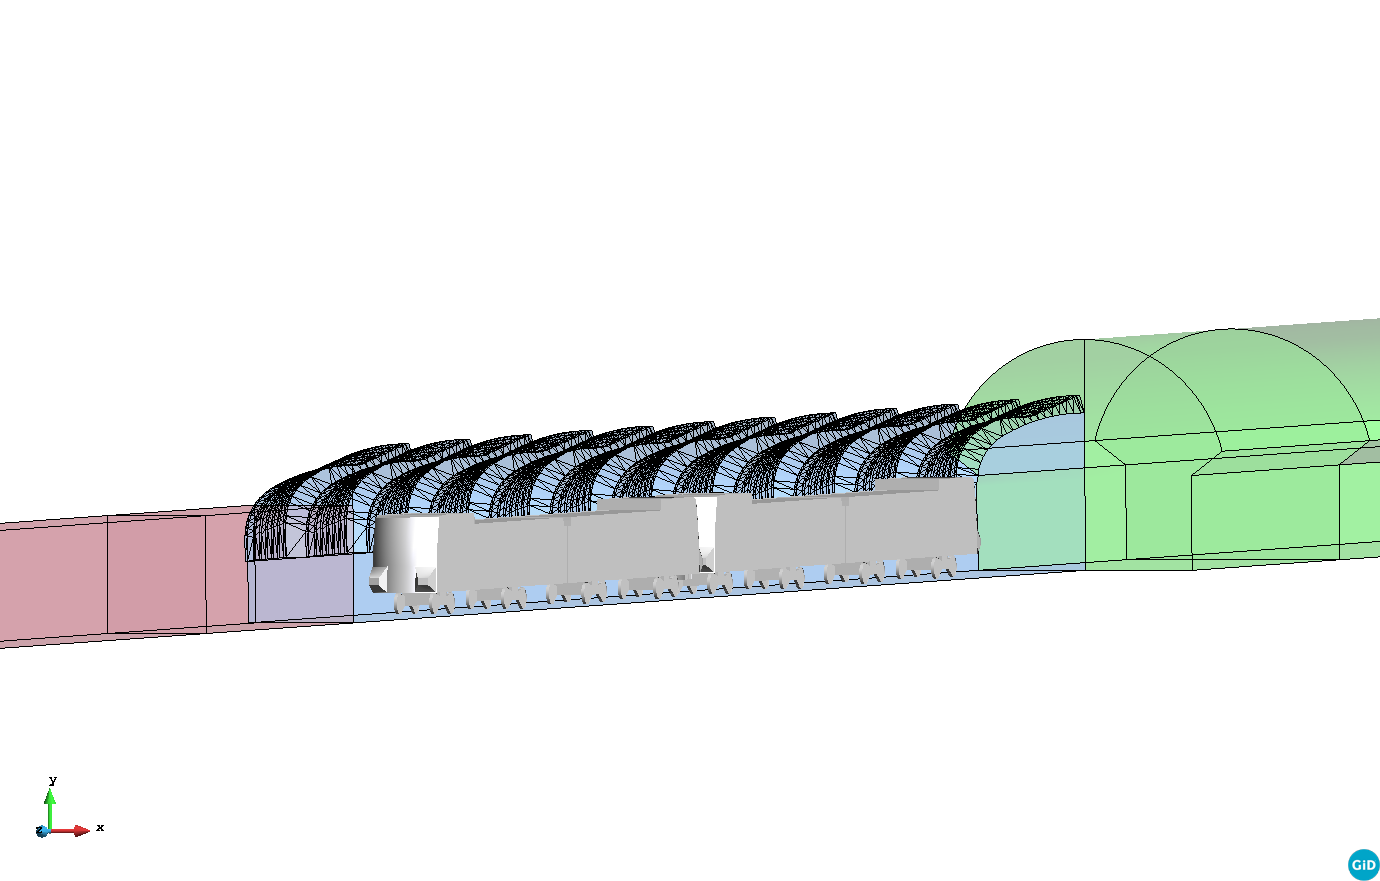
\includegraphics[width=0.8\textwidth,trim={0 7.5cm 0 8.5cm},clip]{figures/ex1-2}
\caption{Train travelling through the middle section of the tunnel.}
\label{fig:Geo2}
\end{figure}

The problem we consider is the circulation of a train through a tunnel, with the particularity that there exists a change in the cross section of this tunnel and the transition between tunnel sections (see \Figu{Geo2}). The objective of the simulation was to evaluate the pressure peaks generated by the train circulation with the aim of structurally designing fire-proof panels in the tunnel wall. This problem fits perfectly in the type of problems described in this paper, as the only possibility to model it is to consider the motion of a solid, the train, inside the tunnel. 

% Add captions to figures
% Describe the problem: main geometry features, main dimensions, boundary conditions,...

The tunnel is composed of three sections: a narrow constant 20 m$^2$ cross-section tunnel, a 95 m long curvy tunnel with average section of 26 m$^2$, and another constant section tunnel of 83 m$^2$. The section of greatest interest is the curvy region in the middle as well as the transition when the train enters this section from the two adjacent ones. The other sections are extended to reduce the impact of boundary conditions at the ends. As a result, the total tunnel length of the computational model is 590 m. 

In the studied case, the train is initially placed in the narrow tunnel section moving at 100 km/h. It travels through the middle curvy section and continues through the wide tunnel. From now on, all physical units are assumed to be given in the SI system. The values of viscosity and density employed are those corresponding to air. 

The surfaces of the train and the tunnel walls are modelled as no-slip boundaries. The ends of the computational domain are in reality sections where the tunnel continues but where the flow is expected to be negligible. Therefore, they are modelled as zero velocity Dirichlet surfaces. This assumption ensures mass conservation and avoids boundary instabilities and it is an approximation to considering a tunnel of infinite length. Furthermore, the length of the computational domain is large enough to ensure that boundary conditions do not impact the flow around the train. The train surface is considered a moving no-slip wall.

% \begin{figure}[h!]
% \centering
% 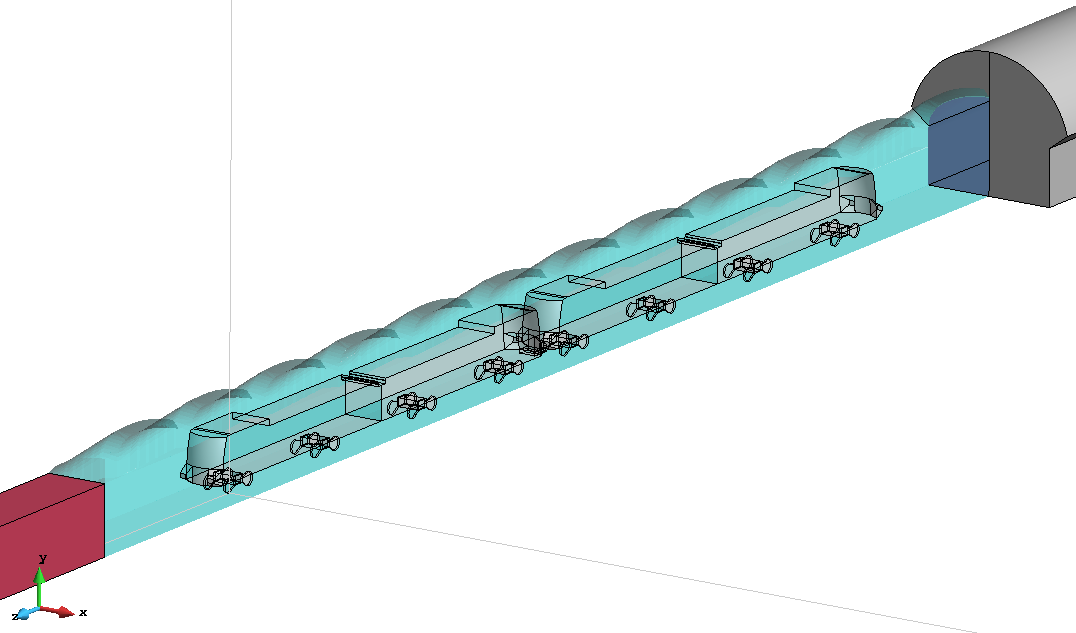
\includegraphics[width=0.5\textwidth]{figures/ex1}
% \caption{ Train travelling through the middle section of the tunnel }
% \label{fig:Geo1}
% \end{figure}

\subsection{Numerical strategy}

% Describe FE mesh, including mesh refinement: elements, sizes, nodes,...

The problem is modelled by embedding a foreground and a background mesh. The foreground mesh contains the geometry of the train and tracks its displacement. The background mesh has the geometry of the air volume inside the tunnel and it is where the computation of the incompressible Navier-Stokes problem takes place. The position and velocity of the train in the foreground mesh is interpolated to the background mesh every time step, where it is imposed as an embedded boundary condition of the aerodynamic problem. Thus, in this case the definition of the solid surface is done through an auxiliary FE mesh.

\begin{figure}[h!]
\centering
    
    \subfloat[Foreground mesh, train\label{fig:MeshFore}]{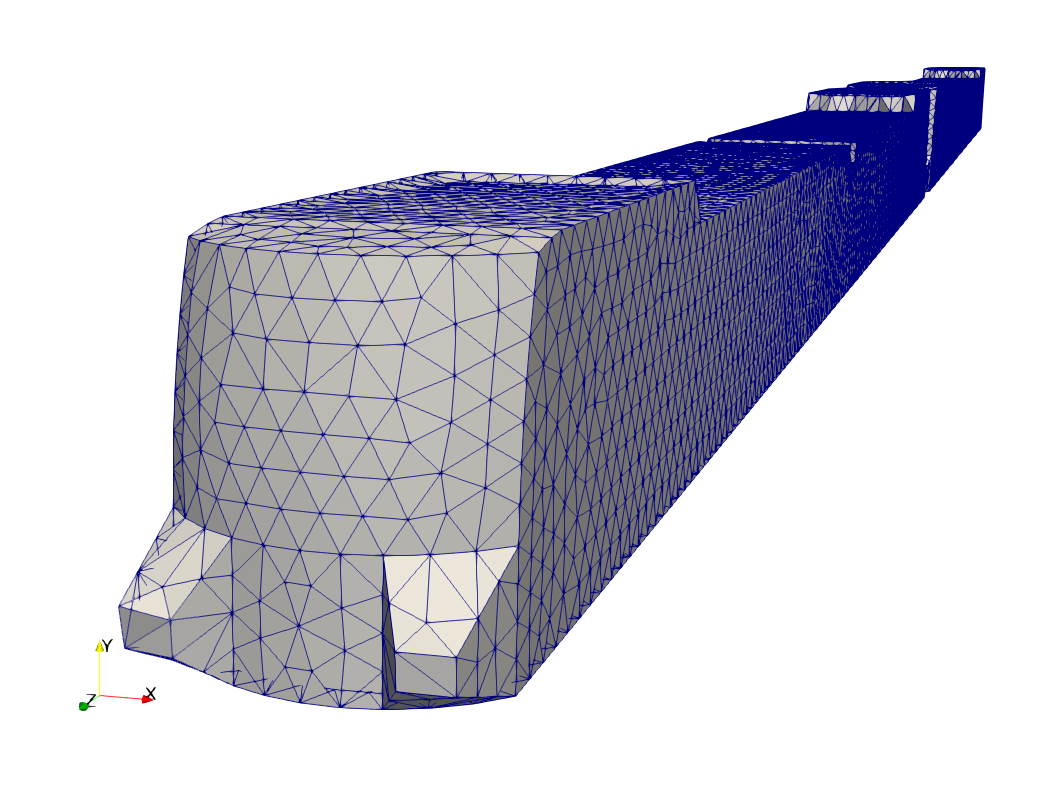
\includegraphics[width=0.5\textwidth]{figures/ex3-2}}
    \subfloat[Background mesh, narrow tunnel\label{fig:MeshBackNarr}]{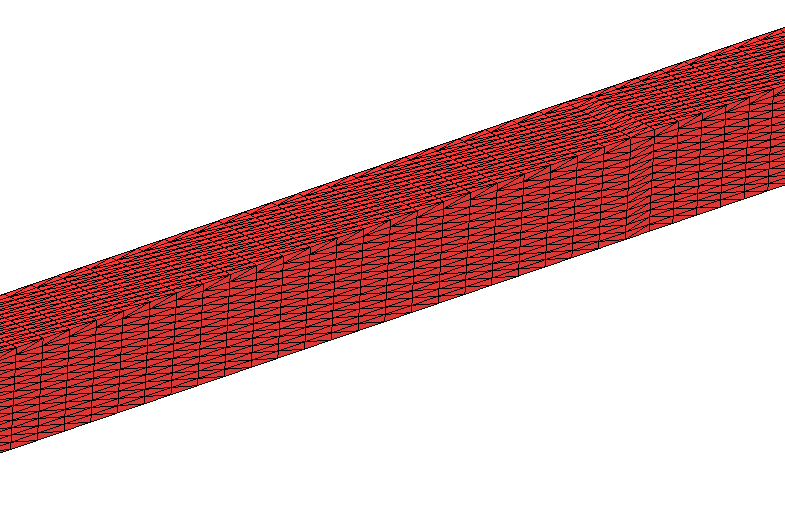
\includegraphics[width=0.5\textwidth]{figures/ex2-3}}
 
    \subfloat[Background mesh, middle curvy tunnel\label{fig:MeshBackMidd}]{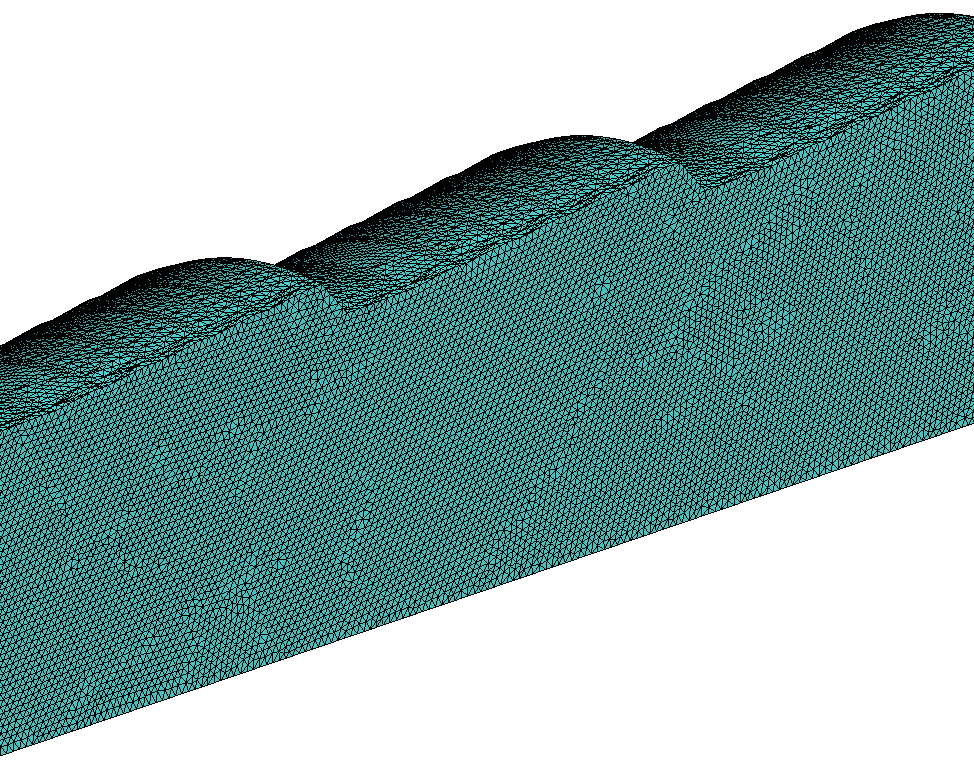
\includegraphics[width=0.5\textwidth]{figures/ex2-2}}
    \subfloat[Background mesh, wide tunnel section\label{fig:MeshBackWide}]{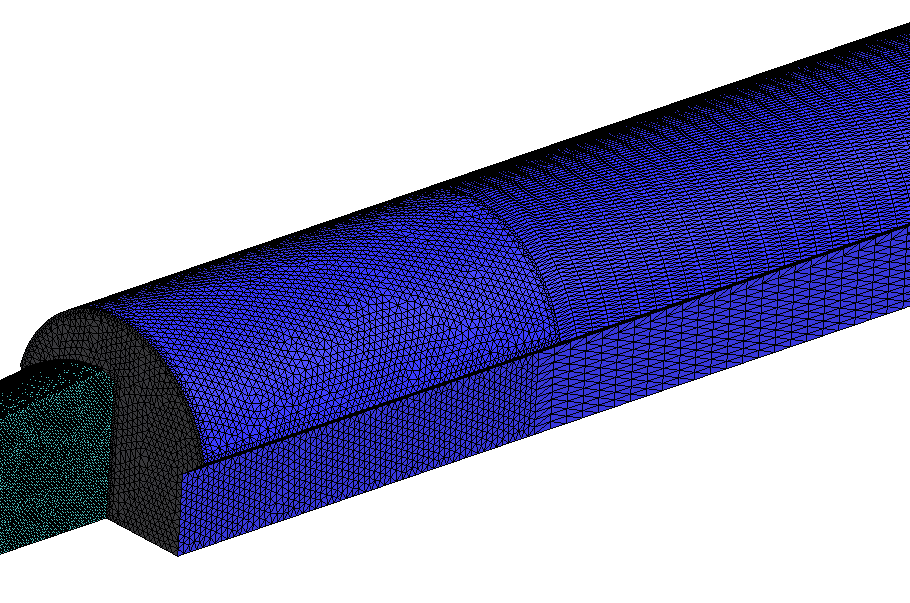
\includegraphics[width=0.5\textwidth]{figures/ex2}}

\caption{Unrefined grid resolution.}
\end{figure}

Two meshes are constructed to model the foreground and the background domains. On the one hand, the foreground mesh focuses on accurately representing the details of the geometry of the train. The foreground mesh has 32702 nodes and 189335 tetrahedral elements, and it is shown in \Figu{MeshFore}.

On the other hand, the background mesh contains the geometry of the tunnel and must comply with the small grid size required by a high-fidelity Navier-Stokes computation. This is achieved by constructing an initial coarse mesh to which adaptive mesh refinement is applied during the computation. While the two tunnel regions with constant section have semi-structured grids generated by extrusion of a surface mesh (see \Figu{MeshBackNarr} and \Figu{MeshBackWide}), the curvy middle section is fully unstructured (\Figu{MeshBackMidd}). Smaller grid size is applied near the tunnel walls to better capture the flow close to the train surface, although it is not our intention to fully capture the turbulent boundary layer. As stated in~\cite{bazilevs-et-al-2007}, Nitche's method when applied to turbulent flows acts as a wall law model. In total, the unrefined background mesh has 2742050 tetrahedral elements and 528493 nodes. In the final computation, adaptive mesh refinement is used on the background mesh. The refinement strategy is based on layers around the surface of the train. In each time step, the 15 layers of elements around the interpolated position of the surface of the train are refined. An additional uniform refinement is also applied. Because the train moves along the tunnel, the refined mesh changes every time step. The refined mesh reached over 60M elements and over 8M nodes.

\begin{figure}[h!]
\centering
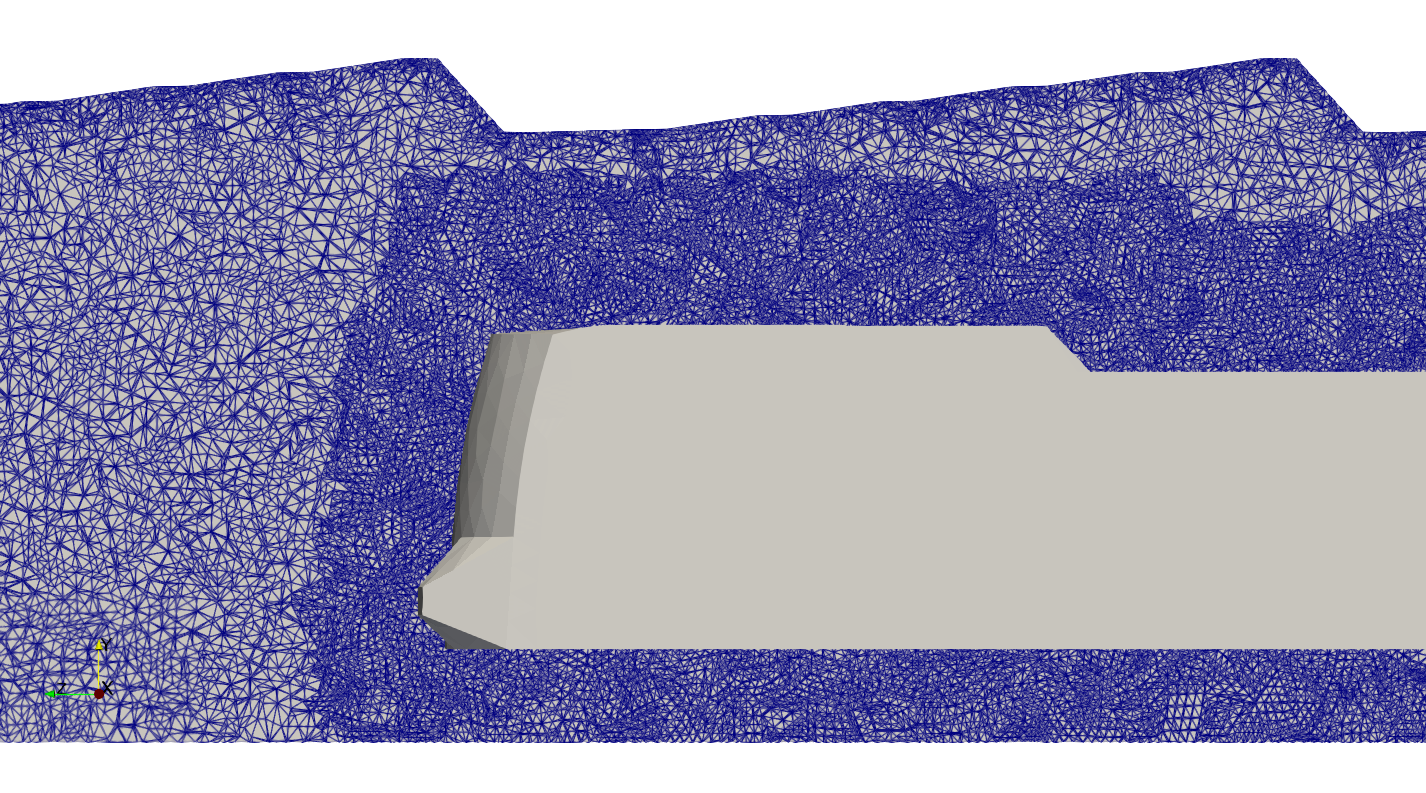
\includegraphics[width=0.5\textwidth]{figures/ex4}
\caption{ Refined background mesh with adaptive refinement around the position of the train.}
\label{fig:MeshRef}
\end{figure}

% Describe relevant numerical parameters: constants of the stabilisation parameters, constants of Nitsche's parameters, constants of the stabilisation of cuts, time step size, time integration scheme...

The computation of the Navier-Stokes problem follows the methodology explained in the previous sections. The background mesh is cut according to the current position of the train surface in the foreground mesh. The velocity of the train is imposed as Dirichlet condition at the cuts. This condition is weakly imposed using Nitsche's method and stabilisation of the cuts. 
%with a penalty parameter $\mu_{\rm N}$ = 10. A constant $\mu_{\rm C}$ = 0.01 is chosen for the stabilisation of the cuts. 
The scheme is stabilised with the following algorithmic parameters for the VMS method: $c_1$ = 4.0 and $c_2$ = 2.0.

The incompressible flow is computed with the fractional step algorithm described in Section~\ref{sec:fs}. In the resolution of the velocity step, 4 Picard (fixed point) iterations are employed. A relaxation factor of 0.8 is used to improve the convergence of the non-linearity.

%In terms of turbulence modelling, LES Smagorinsky with a parameter of 0.01 is used in order to enhance the capturing of turbulent phenomena. 
The artificial compressibility technique is employed, with a parameter of $\beta = 30$, resulting in $c^2  \approx 10^6$. This improves significantly the conditioning of the pressure equation resulting from the fractional step scheme without altering significantly the incompressibility approximation. 

The transient movement of the train takes 7 seconds of physical time. Time integration is done with a second order BDF2 scheme. The problem is computed along 1000 time steps. The chosen time step of $\delta t$= 0.007 is found to be small enough to ensure the nonlinear stability of the implicit integration and to enter the inertial range of the turbulent spectrum.

% Describe parameters from the parallel computation: number of processors, elements per processor...

The computation was carried out on a HPC cluster using 16 Intel Xeon E5-2690v4 processors with a total of 224 CPUs. This represents mesh partitions of around 250000 elements per MPI process, which entails great parallel efficiency according to previous scalability tests. Load rebalancing is also applied to ensure small parallelisation overhead.

Note that the methodology introduced here also works for smaller computations, but the high mesh resolution and the turbulence capturing aimed for this application required the use of a HPC cluster.

\subsection{Numerical results}

\begin{figure}[h!]
\centering
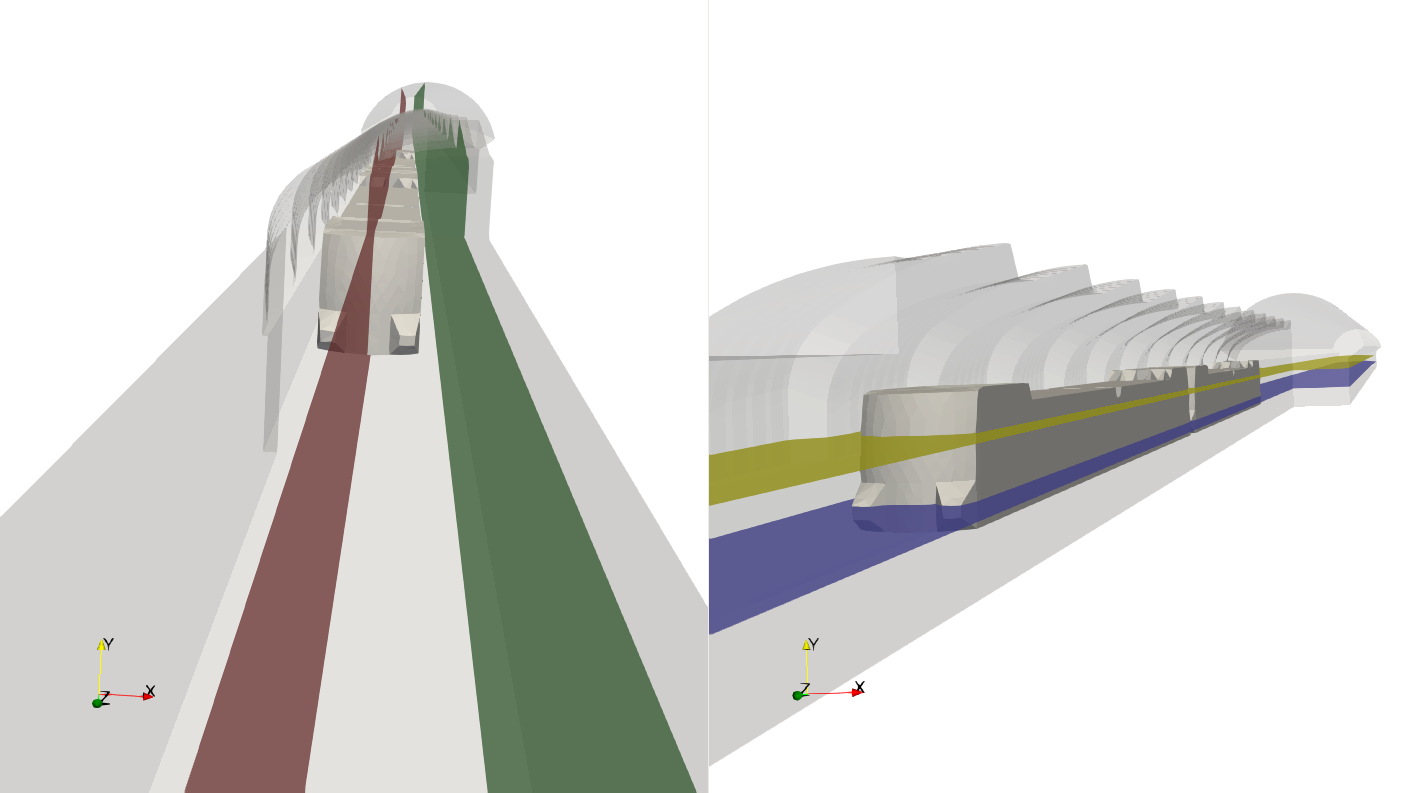
\includegraphics[width=0.7\textwidth]{figures/ex5}
\caption{ Geometry slices where results are presented.}
\label{fig:Slices}
\end{figure}

\begin{figure}[h!]
\centering
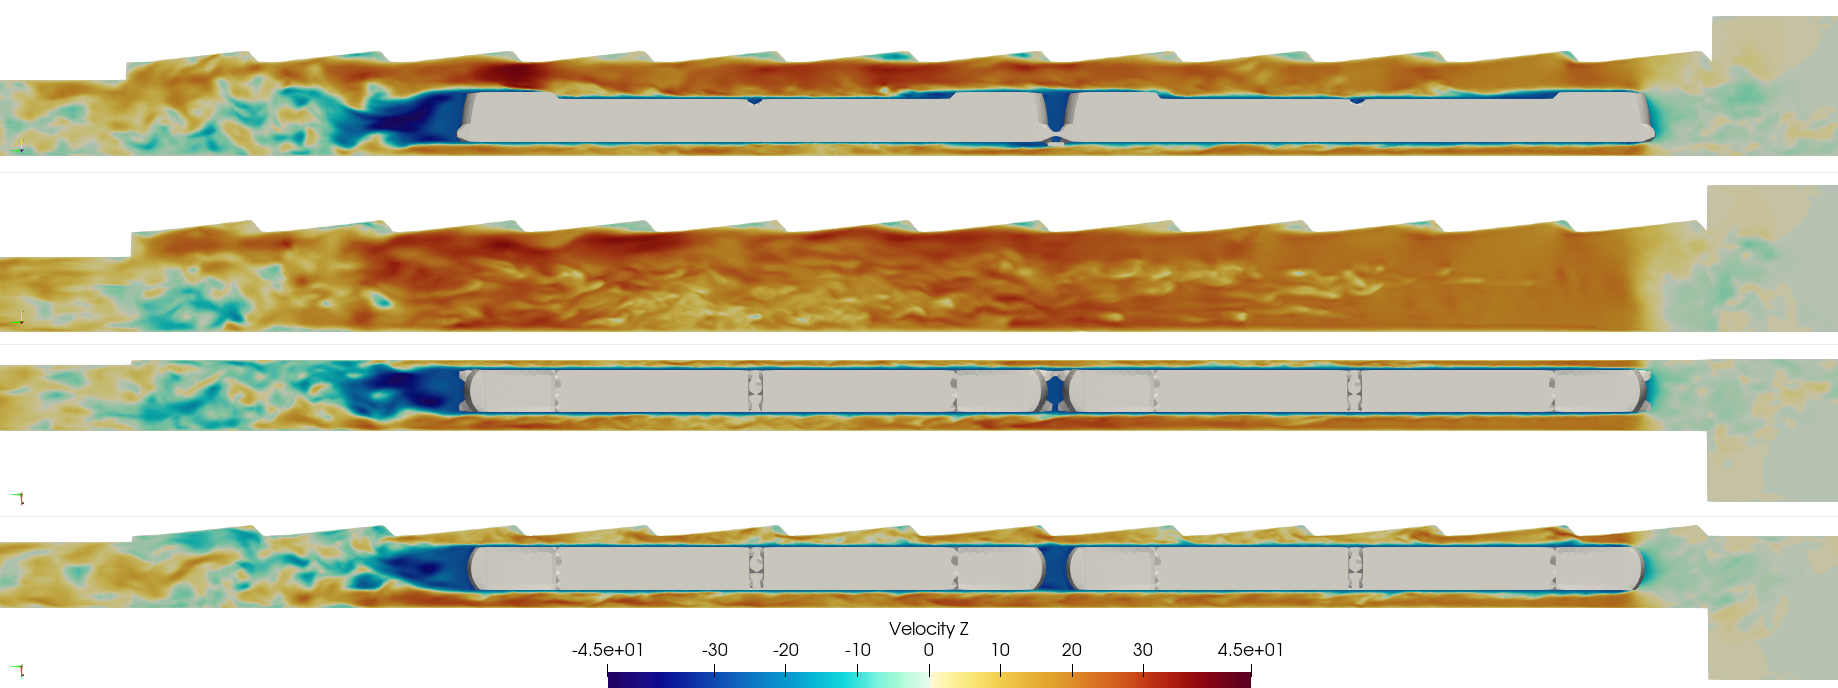
\includegraphics[width=0.85\textwidth,trim={1cm 0 1cm 0},clip]{figures/ex8-2}
\caption{ Slices of lengthwise velocity.}
\label{fig:VelZSlices}
\end{figure}

\begin{figure}[h!]
\centering
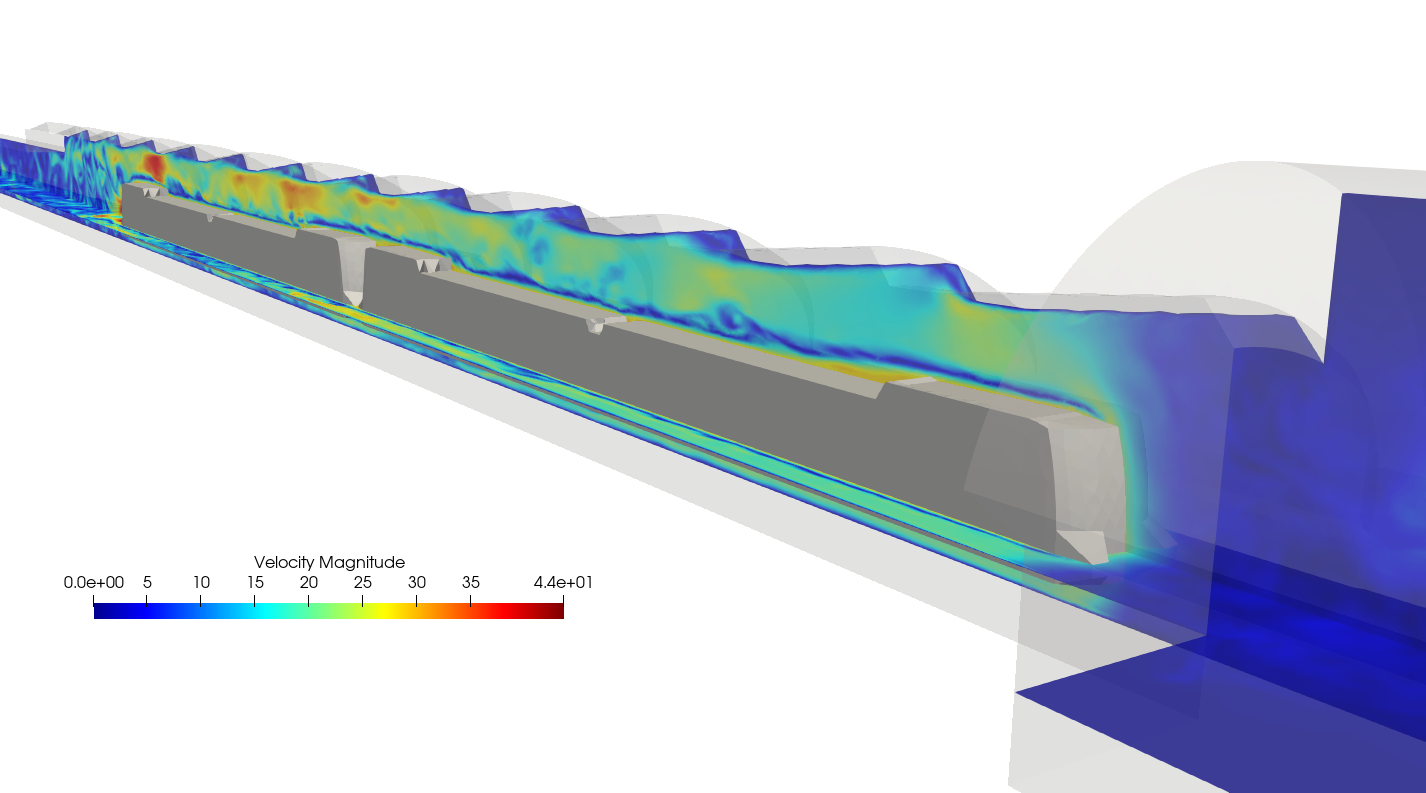
\includegraphics[width=0.85\textwidth,trim={0 6cm 5cm 4.3cm},clip]{figures/ex7}
\caption{ Velocity Magnitude in the tunnel.}
\label{fig:VelMag}
\end{figure}

\begin{figure}[h!]
\centering
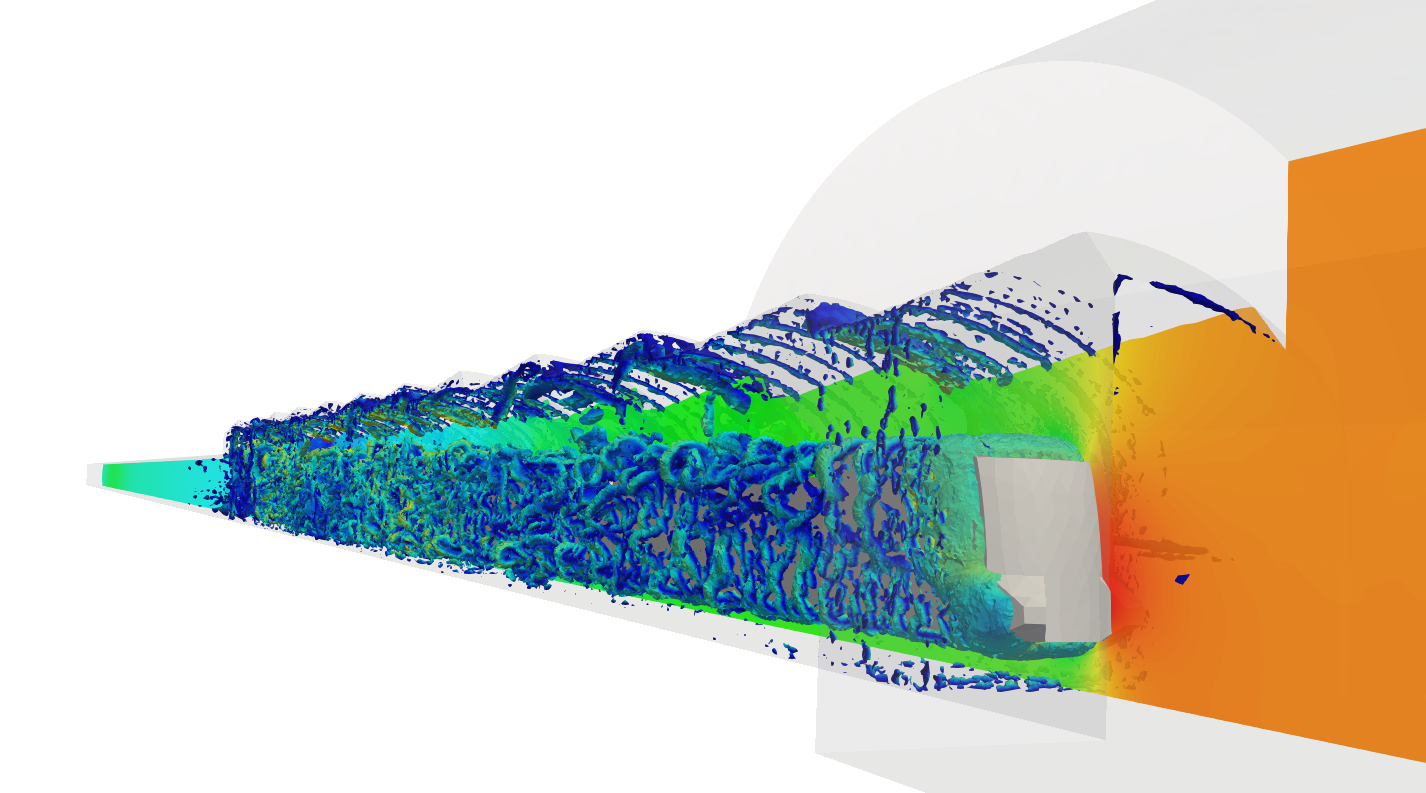
\includegraphics[width=0.85\textwidth,trim={2cm 1cm 2cm 5cm},clip]{figures/ex6}
\caption{ Vortical structures represented with Iso Q-Criterion volumes.}
\label{fig:IsoQ1}
\end{figure}


% \begin{figure}[h!]
% \centering
% 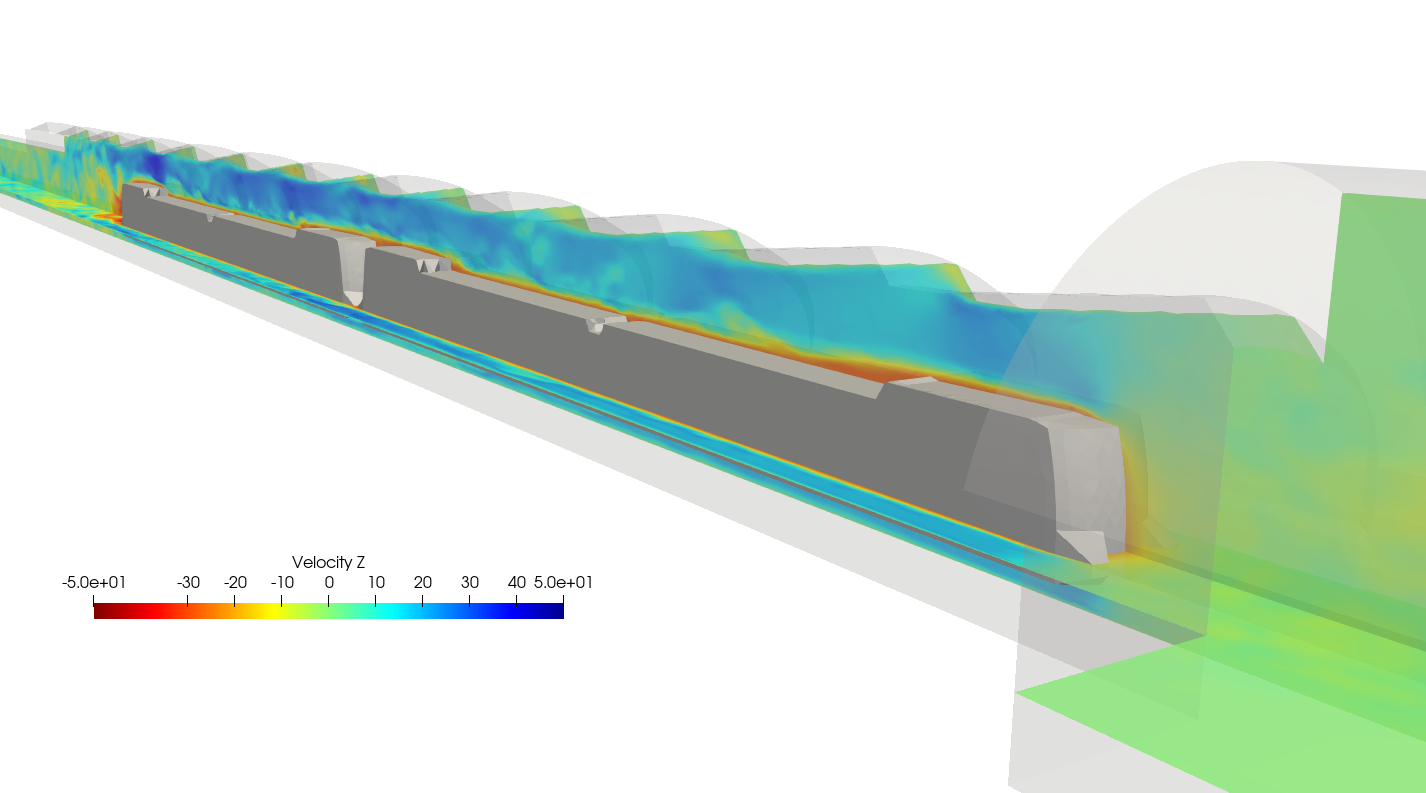
\includegraphics[width=0.95\textwidth,trim={0 6cm 5cm 4.3cm},clip]{figures/ex8}
% \caption{ Lengthwise velocity in the tunnel }
% \label{fig:VelZ}
% \end{figure}

\begin{figure}[h!]
\centering
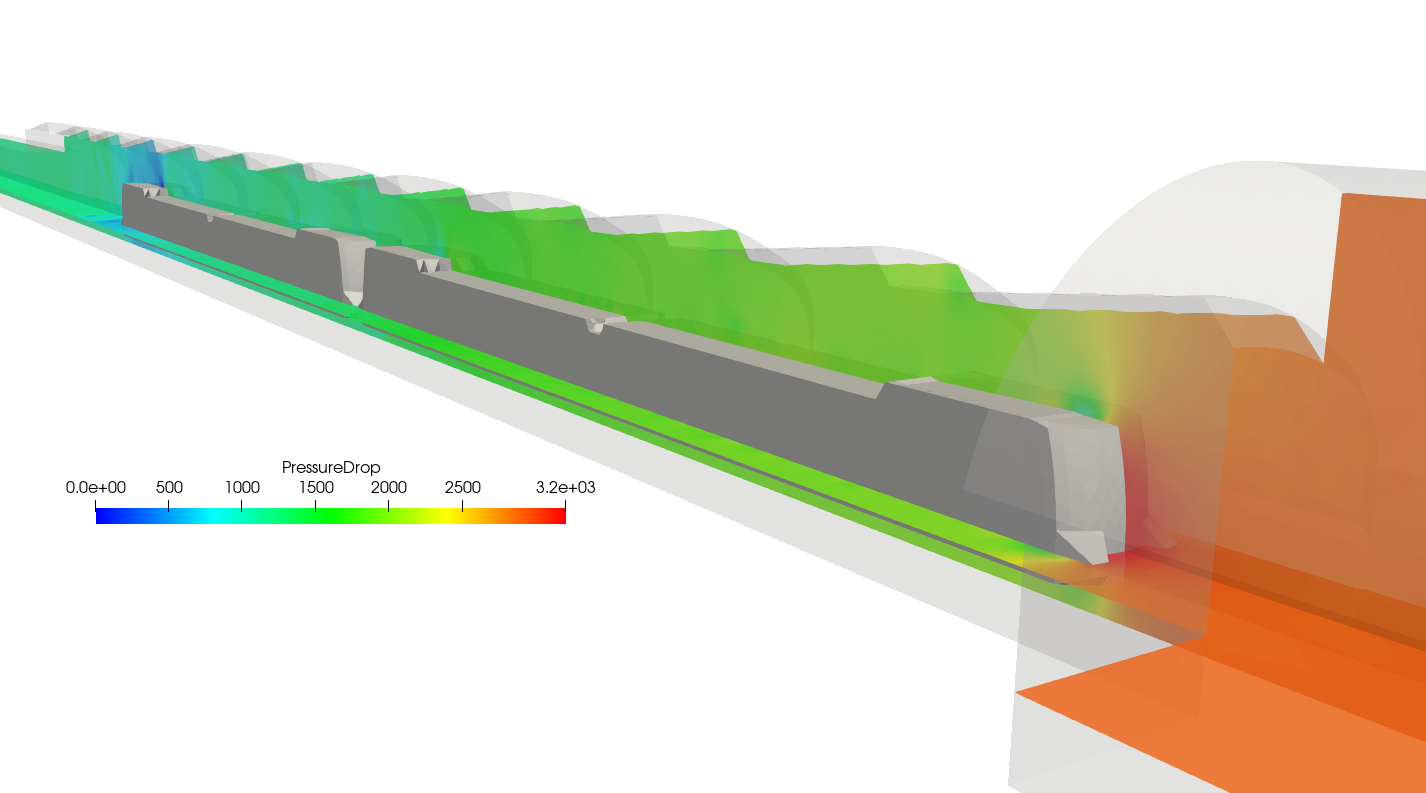
\includegraphics[width=0.85\textwidth,trim={0 6cm 5cm 4.3cm},clip]{figures/ex9}
\caption{ Pressure distribution in the tunnel.}
\label{fig:Pressure}
\end{figure}

\begin{figure}[h!]
\centering
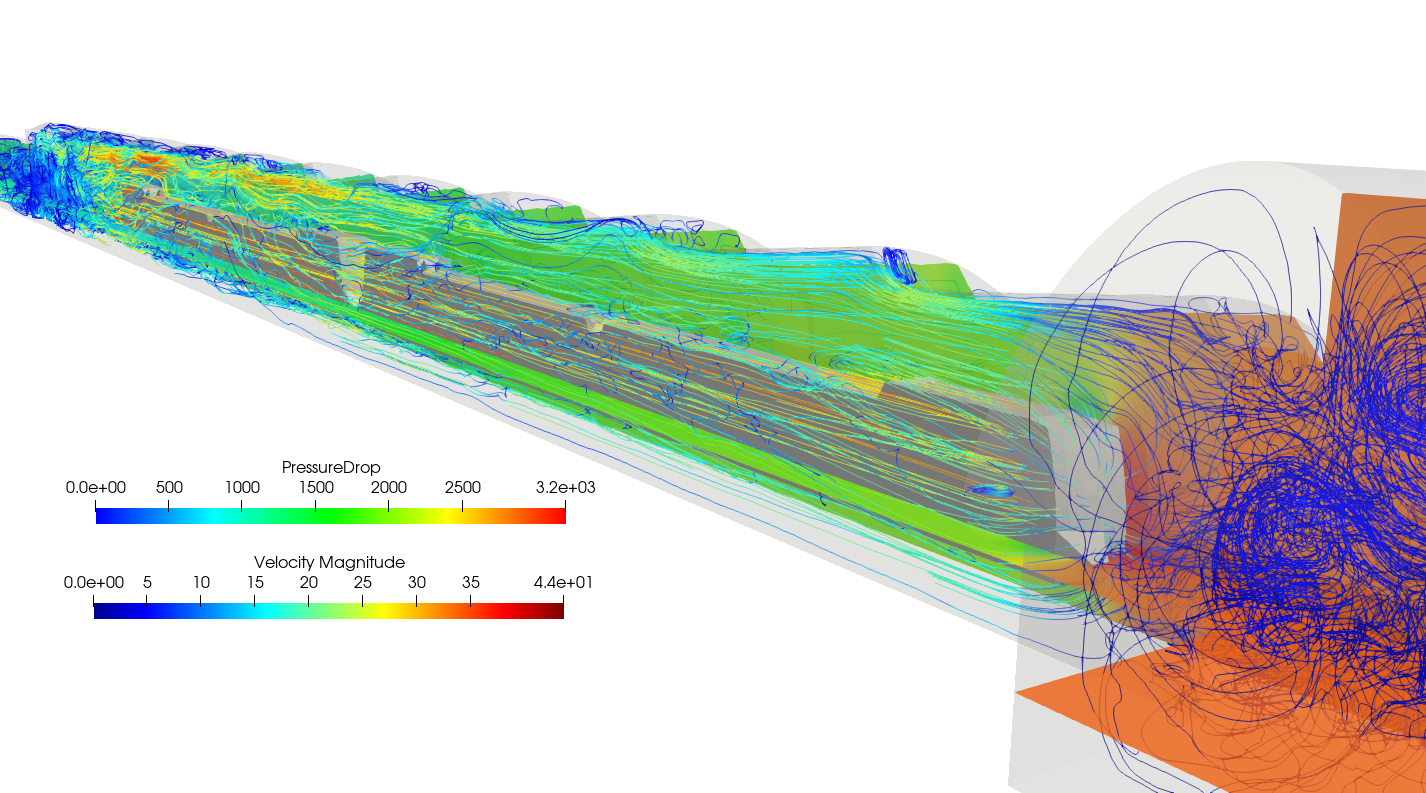
\includegraphics[width=0.85\textwidth,trim={0 6cm 5cm 4.3cm},clip]{figures/ex10}
\caption{ Flow streamlines around the train.}
\label{fig:streamlines}
\end{figure}

% \begin{figure}[h!]
% \centering
% 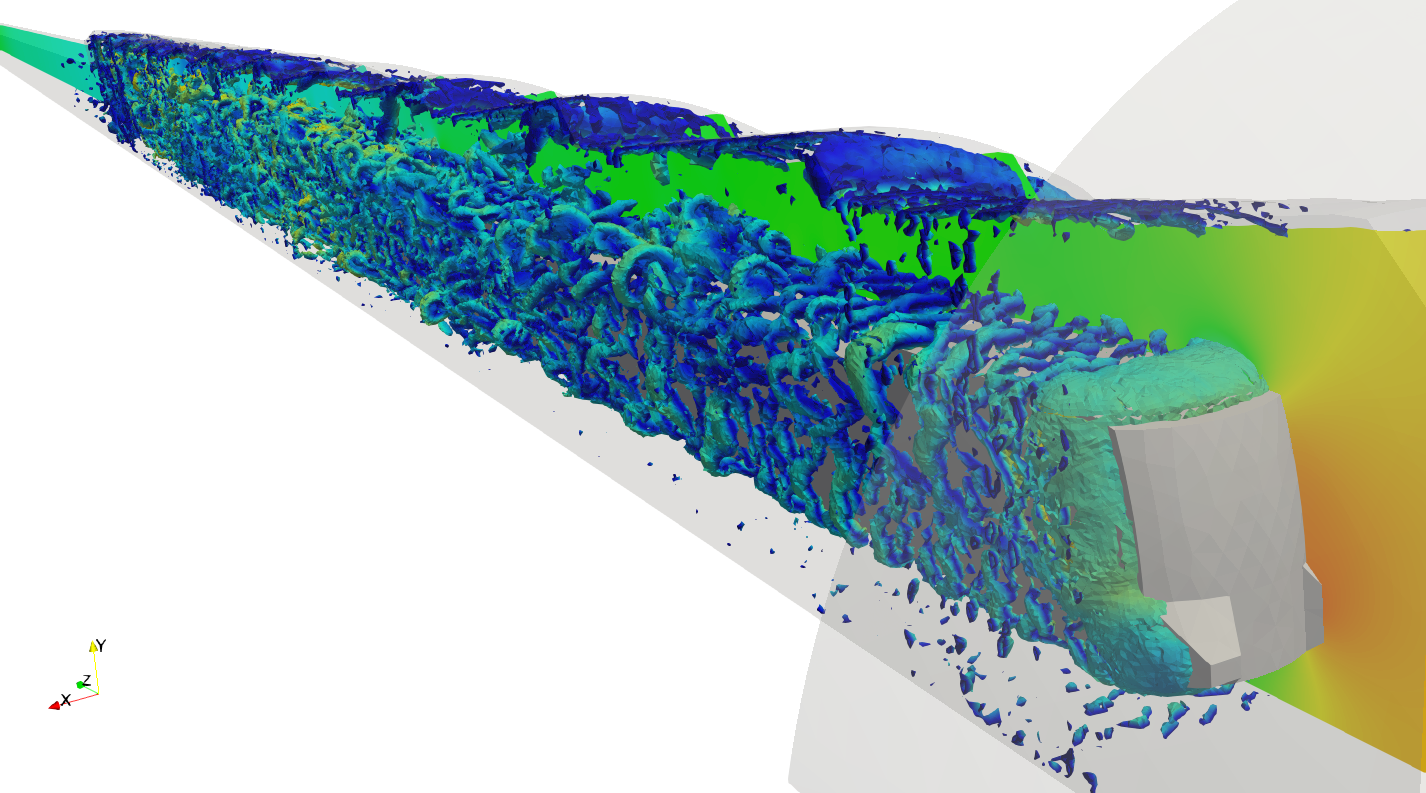
\includegraphics[width=0.95\textwidth]{figures/ex11}
% \caption{ Vortical structures represented with Iso Q-Criterion volumes }
% \label{fig:IsoQ2}
% \end{figure}

% Describe the numerical results

The results presented in this section are taken from an instant when the train is half way through the middle tunnel. The slicing planes used for the representation of results are shown in \Figu{Slices} in the seek of clarity.

% Physical description of the results
% 
As the train moves through the tunnel, it drags along a layer of air through shear stresses (see \Figu{VelZSlices}). The displaced air from ahead travels in the opposite direction in the gap between the train and the tunnel walls (\Figu{VelMag}). The problem is characterised by strong turbulent flow (\Figu{IsoQ1}). The flow detaches at the nose of the train creating vortices on both sides. Secondary vortices develop all along the sides of the train. Additional vortices are generated when the flow hits the sharp edges of the tunnel walls. Turbulence is greatest at the tail of the train, where vortices are alternatively detached as air from the sides of the train is sucked. As a result, the train leaves behind a wake region which gradually dissipates downstream. As expected, the maximum pressure is found at the nose of the train and the strongest suction appears at the tail (see \Figu{Pressure} and \Figu{streamlines}). There is a pressure drop along the sides of the train.


% Numerical description of the results
The results show a fluid problem computation with a high level of detail. The fine discretisation allows for the resolution of a large range of turbulent scales, leading to an accurate capturing of the eddies and complex features of the flow. The implemented embedded methodology achieved the task of transferring the position and velocity of the train, enabling the resolution of a fully transient and complicated problem which would have been very difficult to solve with a single fixed mesh or with a classical ALE approach.
 
% Adaptivity
The adaptive mesh refinement (\Figu{MeshRef}) also plays a significant role in the numerical computation. Firstly, it provides the background mesh with fine element sizes 
in the region close to the surface of the train. This optimises the imposition of boundary conditions, thus enhancing the precision of the embedded strategy. Secondly, it refines the region around the train where the most complex flow features appear. This guarantees a mesh resolution capable of capturing sharp gradients and turbulent phenomena, even if we have not aimed at fully capturing the boundary layer, while the regions further from the train where the flow is smooth and easily computed remain unrefined. As a result, the refinement strategy proves to be successful in increasing the accuracy of the numerical scheme and the computational efficiency.

\subsection{Numerical performance}

% Give information about the performance of the iterative scheme: mean number of iterations, maximum, minimum, tolerance reached...
% Give information about the iterative solver: iterations of the different equations, CPU (in % with respect to the total of a time step, for example), tolerance reached,... Comment about the possible cost of a monolithic scheme (considering that the number of iterations would be that of the pressure).

The computation of the whole problem with 224 CPUs took 35 h. 90\% of the computation time was spent on the assembly and solving of the linear systems of the different steps of the incompressible Navier-Stokes fractional step algorithm. The velocity step non-linearity converged to the order of $10^{-3}$ with 4 Picard iterations.

%\begin{table}[]
%\caption{Performace of the solver of the fractional step algorithm for a representative time step.}
%\label{tab:Solver}
%\begin{tabular}{lccc}
%\textbf{Problem [Picard iteration]}       & \multicolumn{1}{l}{\textbf{Solver iterations}} & \multicolumn{1}{l}{\textbf{Solver residual}} & \multicolumn{1}{l}{\textbf{Solver Time}} \\
%Velocity [1]          & 140                                     & 2.31$\times 10^{-6}$                                & 18.3 s                                  \\
%Velocity [2]          & 135                                     & 4.01$\times 10^{-6}$                                & 17.5 s                                  \\
%Velocity [3]          & 136                                     & 3.32$\times 10^{-6}$                                & 17.6 s                                  \\
%Velocity [4]          & 141                                     & 4.17$\times 10^{-6}$                                & 18.1 s                                  \\
%Pressure Correction & 574                             & 1.15$\times 10^{-6}$                                  & 31.5 s                                 
%\end{tabular}
%\end{table}

\begin{table}[]
\caption{Performace of the solver of the fractional step algorithm for a representative time step.}
\label{tab:Solver}
\begin{tabular}{lcc}
\textbf{Problem [Picard iteration]}       & \multicolumn{1}{l}{\textbf{Solver iterations}} & \multicolumn{1}{l}{\textbf{Solver Time}} \\
Velocity [1]          & 140                                     & 18.3 s                                  \\
Velocity [2]          & 135                                     & 17.5 s                                  \\
Velocity [3]          & 136                                     & 17.6 s                                  \\
Velocity [4]          & 141                                     & 18.1 s                                  \\
Pressure Correction & 574                               & 31.5 s                                 
\end{tabular}
\end{table}


In terms of solver of the linear systems, the parallel library PETSc was employed \cite{PETScHomePage}. The iterative BCGs (Biconjugate Gradients Stabilized) \cite{BiconjugateGradientSolver} solver with ILU preconditioner was chosen for this problem. The convergence of the solver was stable, typically reaching a tolerance of the order of $10^{-6}$. The linear solver of the fluid problem used a 73\% of the total CPU time. The solver information for a characteristic step is found in Table~\ref{tab:Solver}.

It is interesting to notice the high number of iterations and time required for the pressure correction step compared to a velocity step. Had a monolithic algorithm been used instead of the proposed fractional step, the solver of the monolithic system would have taken at least the iterations required by the pressure correction step, creating a significant computation overhead. Considering that each nonlinear iteration would involve four variables per node instead of three (pressure plus three velocity components), and that the number iterations would be driven by the pressure (of the order of 574 instead of something between 135 and 141), the expected factor of CPU increase would be about 5.5. 

It is interesting to point out that the adaptive refinement uses 1.8\% of the computation time and the embedding operations take 1\%. The computation overhead of both is negligible compared to solving of the incompressible Navier-Stokes systems. This justifies the use of the different ingredients of the methodology and proves its numerical efficiency.

\section{Conclusions}\label{sec:conclu}

In this paper we have presented a methodology to deal with large scale fluid flow problems in which the flow domain changes because of the motion of a solid moving inside a fluid. The novelties of the paper consist of the tailoring of different numerical techniques to this problem and also two specific new ingredients. The former include a stabilised FE method that can be used as implicit LES, the fixed-mesh ALE strategy, the weak imposition of boundary conditions in non-matching meshes, the artificial compressibility technique and the adaptive mesh refinement, whereas the latter are the stabilisation of badly cut elements and the design of the fractional step scheme. In all cases, the choice of these techniques is motivated by the physical needs and, above all, by efficiency considerations. This is why we favour for example fractional step schemes rather than monolithic ones and fixed mesh methods rather than moving meshes.

The resulting formulation is very robust and efficient. We have presented a numerical simulation with the objective of highlighting the convenience of the choices adopted and the good numerical performance of this formulation, both from the point of view of the quality of the results and from the computational efficiency. 

\section*{Acknowledgements}

R. Codina gratefully acknowledges the support received through the ICREA Acad\`emia Research Program of the Catalan Government. 
I. Casta\~nar gratefully acknowledges the support received from the Ag\`encia de Gesti\'o d'Ajuts i de Recerca through the predoctoral FI grant 2019-FI-B-00649.
%L. Moreno acknowledges the support received from the project Nemesis, LARE\_BIRD2020\_01 (id: 33593). 
CIMNE is a recipient of a ``Severo Ochoa Programme for Centers of Excellence in R\&D'' grant (CEX2018-000797-S) by the Spanish Ministry of Economy and Competitiveness.
   
\bibliographystyle{ieeetr}
%\bibliographystyle{plain}
\bibliography{latexbi}

\end{document}
